%\documentclass[a4paper,12pt,twoside]{book}
\documentclass[listof=nochaptergap,12pt,times,authoryear]{report}
\usepackage{mathptmx}%This package supersedes times and mathptm
\usepackage[a4paper,right=2.54cm,left=2.54cm,top=2.54cm,bottom=2.54cm]{geometry}
\usepackage{array}
\usepackage{listings}
\usepackage{pdflscape}
\usepackage{longtable}
\usepackage{enumitem}
\usepackage{newclude}
\usepackage{float}
\usepackage{comment}
\usepackage[export]{adjustbox}
\usepackage{algorithm}
\usepackage{algpseudocode}

\floatname{algorithm}{Algoritmo}

\newcolumntype{C}[1]{>{\centering\arraybackslash}p{#1}}
\newcolumntype{N}{@{}m{0pt}@{}}
\newcommand\fillin[1][3cm]{\makebox[#1]{\dotfill}}

%%Paquete para ocultar indices de tabla de contenidos
%% Numeración continua en figuras y tablas
\setcounter{equation}{0}
\usepackage{chngcntr}
\counterwithout{figure}{chapter}
\counterwithout{table}{chapter}
\counterwithout{equation}{chapter}
\renewcommand{\thefigure}{\arabic{figure}}
\renewcommand{\thetable}{\arabic{table}}
\renewcommand{\theequation}{\arabic{equation}}

% Parche para eliminar espacios por capítulos en lista de figuras y tablas
\usepackage{etoolbox}% http://ctan.org/pkg/etoolbox
\makeatletter
% \patchcmd{<cmd>}{<search>}{<replace>}{<succes>}{<failure>}
\patchcmd{\@chapter}{\addtocontents{lof}{\protect\addvspace{10\p@}}}{}{}{}% LoF
\patchcmd{\@chapter}{\addtocontents{lot}{\protect\addvspace{10\p@}}}{}{}{}% LoT
\makeatother


%%%%paquete para usar citas de diferentes formatos
%%%%%%%%%%%%%%%%%%%%%%%%%%%%%%%%%
%%add al indice
%\usepackage[nottoc,numbib]{tocbibind}
%\usepackage[authoryear,round]{natbib}
\usepackage[utf8]{inputenc}
\usepackage{csquotes}
\usepackage[spanish,es-lcroman]{babel}
\decimalpoint
%% Citas y bibliografía formato APA
\usepackage[backend=biber,style=apa,natbib=true]{biblatex}
%\DeclareLanguageMapping{australian}{australian-apa}
\DeclareLanguageMapping{spanish}{spanish-apa}
\addbibresource{biblio/references.bib}

%% Formato DOI
\DeclareFieldFormat{doi}{%
	doi\addcolon\space
	\ifhyperref
	{\lowercase{\href{https://doi.org/#1}{\nolinkurl{#1}}}}
	{\lowercase{\nolinkurl{#1}}}}

%% Formato de URL en referencias
\DeclareFieldFormat{url}{{Recuperado de}\space\url{#1}}

%% Convertir comando cita por textcite para que tenga formato APA
\let\cite\textcite

%% Para que texto de figuras y tablas tenga formato APA
\usepackage{multirow,booktabs,setspace,caption}
\DeclareCaptionLabelSeparator*{spaced}{\\[2ex]}
\captionsetup[table]{labelfont=normalfont,textfont=it,format=plain,justification=justified,singlelinecheck=false,labelsep=newline,skip=2pt}
\captionsetup[figure]{labelsep=period,labelfont={it,bf},justification=justified,singlelinecheck=false,font=doublespacing}
\captionsetup[subfigure]{justification=centering}

%%%Editar formato y tamaño de capítulos y secciones
\usepackage{titlesec}
\titleformat{\chapter}
{\centering\normalfont\large\bfseries}{Capítulo \thechapter:}{1em}{}
\titlespacing*{\chapter}{0pt}{-4ex}{1ex}

\titleformat{\section}
{\normalfont\large\bfseries}{\thesection}{1em}{}
\titlespacing*{\section}{0pt}{0pt}{0pt}

\titleformat{\subsection}
{\normalfont\large\bfseries}{\thesubsection}{1em}{}
\titlespacing*{\subsection}{0pt}{0pt}{0pt}

%\usepackage{biblatex}
%paquete para hiperlinks entre citas e imagenes
%%%%%%%%%%%%%%%%%%%%%%%%%%%%%%%%%
\usepackage[colorlinks=true,
citecolor=black,
urlcolor=black,
bookmarks=true,
linkcolor=black,
pdftitle={Diseño de un sistema de gestion inteligente de semaforos aplicando aprendizaje por refuerzo en el municipio de Santiago de Surco
},
pdfauthor={Diego Alonso La Torre Echegaray}]{hyperref}

\usepackage{amssymb}
\usepackage{graphicx} % for improved inclusion of graphics
%\usepackage{wrapfig} % to include figure with text wrapping around it
\usepackage[margin=10pt,font=small,labelfont=bf]{caption} % for improved layout of figure captions with extra margin, smaller font than text
\usepackage{subcaption}
\usepackage{eucal}
\usepackage[usenames, dvipsnames]{color}
\usepackage[perpage]{footmisc}
%\usepackage[round, sort]{natbib}
\usepackage{ifthen}
\usepackage{multicol} % for pages with multiple text columns, e.g. References
\setlength{\columnsep}{20pt} % space between columns; default 10pt quite narrow
%% Para no mostrar índices de figuras ni tablas en el índice general
\usepackage[nottoc,notlot,notlof]{tocbibind}
%\usepackage{appendix}
\usepackage[titletoc,title]{appendix} 

%%%----Modificar encabezado y pie de pagina
%%%%%%%%%%%%%%%%%%%%%%%%%%%%%%%%%%%%%%%%%%%%%%%%%%%%%%%%%%%%%%%%%%%%%
\usepackage{fancyhdr} % for better header layout
\newcommand{\changefont}{%
	\fontsize{9pt}{1.5pt}\selectfont
}

\pagestyle{fancy}
%%Para borrar fancy por default (incluye numeracion)
\fancyhf{} % sets both header and footer to nothing
%%Para borrar linea de encabezado
\renewcommand{\headrulewidth}{0pt}
%%Encabezados solo con numero de pagina
\fancypagestyle{normal}{%
	\fancyhead{} % clear all header fields
	\fancyhead[R]{\thepage}}
%%Encabezados con titulo de tesis y numero de pagina
\fancypagestyle{special}{%
	\fancyhead[L]{\changefont Diseño de un sistema de gestion inteligente de semaforos aplicando aprendizaje por refuerzo en el municipio de Santiago de Surco}
	\fancyhead[R]{\thepage}}


%\fancyhf{} %% delete default configuration of page
%%\setlength\headheight{15pt}

%%%%%%%%%%%%%%%%%%%%%%%%%%%%%5
%%%% Configuracion de los parrafos
%\usepackage{setspace}
%\onehalfspacing 
\setlength{\parindent}{0.5in} %%sangria
\setlength{\parskip}{3mm}  %%espacio entre parrafos
\linespread{1.3} %This equals 1.5 linespacing in Word
%%%% nuevo parrafo
%%%%%%%%%%%%%%%%%%%%%%%%%%%%%5
%%%% Centrar valores de una tabla
\usepackage{array}
%%CENTRADO HORIZONTAL
\newcolumntype{P}[1]{>{\centering\arraybackslash}p{#1}}
%%CENTRADO VERTICAL
\newcolumntype{M}[1]{>{\centering\arraybackslash}m{#1}}

%%%%%%%%%%%%%%%%%%%%%%%%%%%%%5
%%%%Paquete para alinear texto
\usepackage{ragged2e}
\usepackage{multirow}
\usepackage{makecell}
\usepackage{rotating}
\usepackage{siunitx} % To align the numbers later on
\usepackage[table,xcdraw]{xcolor}
\usepackage{color, colortbl}
\definecolor{Gray}{gray}{0.9}
\definecolor{orange}{rgb}{1,0.647,0}
\definecolor{turq3}{rgb}{0.54, 0.81, 0.94}
\definecolor{turq}{rgb}{0.63, 0.79, 0.95}
\definecolor{bluejean}{rgb}{0.03, 0.27, 0.49}

%%%%%%%%%%%%%%%%%%%%%%%%%
\usepackage{xparse}
\usepackage{expl3}
%%%%funcion de reemplazar regex
\ExplSyntaxOn
\NewDocumentCommand{\replace}{mmm}
{
	\marian_replace:nnn {#1} {#2} {#3}
}

\tl_new:N \l_marian_input_text_tl
\tl_new:N \l_marian_search_tl
\tl_new:N \l_marian_replace_tl

\cs_new_protected:Npn \marian_replace:nnn #1 #2 #3
{
	\tl_set:Nn \l_marian_input_text_tl { #1 }
	\tl_set:Nn \l_marian_search_tl { #2 }
	\tl_set:Nn \l_marian_replace_tl { #3 }
	\regex_replace_all:nnN { \b\u{l_marian_search_tl}\b } { \u{l_marian_replace_tl} } \l_marian_input_text_tl
	\tl_use:N \l_marian_input_text_tl
}
\ExplSyntaxOff

%%%%%%%%%%%%%%%%%%%%%%%%%%%%%%%%%%%%%%
\usepackage{amsmath}
%\setcounter{equation}{0}
%\numberwithin{equation}{chapter} %%enumerar ecuaciones
%\renewcommand{\theequation}{Ecuación \arabic{equation}}   
\usepackage{mathtools, nccmath, cool}
%%%Configuraciones de biblatex

%%%hel
%%%%\citeauthor
\makeatletter

%%%%%%%%%%%%
\DeclareCiteCommand{\citeauthor}
{\boolfalse{citetracker}%
	\boolfalse{pagetracker}%
	\usebibmacro{prenote}}
{\ifciteindex
	{\indexnames{labelname}}
	{}%
	\printtext[bibhyperref]{\printnames{labelname}}}
{\multicitedelim}
{\usebibmacro{postnote}}


\DeclareCiteCommand{\citetitle}
{\boolfalse{citetracker}%
	\boolfalse{pagetracker}%
	\usebibmacro{prenote}}
{\ifciteindex
	{\indexfield{indextitle}}
	{}%
	\printtext[bibhyperref]{\printfield[citetitle]{labeltitle}}}
{\multicitedelim}
{\usebibmacro{postnote}}

\DeclareCiteCommand{\cite}
{\usebibmacro{prenote}}
{\usebibmacro{citeindex}%
	\printtext[bibhyperref]{\usebibmacro{cite}}}
{\multicitedelim}
{\usebibmacro{postnote}}

\DeclareCiteCommand*{\cite}
{\usebibmacro{prenote}}
{\usebibmacro{citeindex}%
	\printtext[bibhyperref]{\usebibmacro{citeyear}}}
{\multicitedelim}
{\usebibmacro{postnote}}

\DeclareCiteCommand{\parencite}[\mkbibparens]
{\usebibmacro{prenote}}
{\usebibmacro{citeindex}%
	\printtext[bibhyperref]{\usebibmacro{cite}}}
{\multicitedelim}
{\usebibmacro{postnote}}

\DeclareCiteCommand*{\parencite}[\mkbibparens]
{\usebibmacro{prenote}}
{\usebibmacro{citeindex}%
	\printtext[bibhyperref]{\usebibmacro{citeyear}}}
{\multicitedelim}
{\usebibmacro{postnote}}

\DeclareCiteCommand{\footcite}[\mkbibfootnote]
{\usebibmacro{prenote}}
{\usebibmacro{citeindex}%
	\printtext[bibhyperref]{ \usebibmacro{cite}}}
{\multicitedelim}
{\usebibmacro{postnote}}

\DeclareCiteCommand{\footcitetext}[\mkbibfootnotetext]
{\usebibmacro{prenote}}
{\usebibmacro{citeindex}%
	\printtext[bibhyperref]{\usebibmacro{cite}}}
{\multicitedelim}
{\usebibmacro{postnote}}

\DeclareCiteCommand{\textcite}
{\boolfalse{cbx:parens}}
{\usebibmacro{citeindex}%
	\printtext[bibhyperref]{\usebibmacro{textcite}}}
{\ifbool{cbx:parens}
	{\bibcloseparen\global\boolfalse{cbx:parens}}
	{}%
	\multicitedelim}
{\usebibmacro{textcite:postnote}}
\makeatother
\makeatletter
\let\abx@macro@citeOrig\abx@macro@cite
\renewbibmacro{cite}{%
	\bibhyperref{%
		\let\bibhyperref\relax\relax%
		\abx@macro@citeOrig%
	}%
}
\let\abx@macro@textciteOrig\abx@macro@textcite
\renewbibmacro{textcite}{%
	\bibhyperref{%
		\let\bibhyperref\relax\relax%
		\abx@macro@textciteOrig%
	}%
}%

\makeatother

%%%%%%%%%%%%%%%%%%%%%%%%%%%%%%%%%%%%%%%%%%%
% Agregando librerias para que aparezca texto debajo de las ecuaciones.
\usepackage[titles]{tocloft}

%% Para agregar palabra "CAPÍTULO" en 
\newlength\mynewlength
\let\oldcftchappresnum\cftchappresnum
\renewcommand*\cftchappresnum{Capítulo \oldcftchappresnum}
\renewcommand\cftchapaftersnum{:}
\settowidth\mynewlength{\cftchappresnum\cftchapaftersnum\quad}
\addtolength\cftchapnumwidth{\mynewlength}

\usepackage{xpatch}
\usepackage{caption}
\DeclareCaptionType{equcaption}[Ecuación][Índice de Ecuaciones]

\newenvironment{conditions}
{\par\vspace{\abovedisplayskip}\noindent\begin{tabular}{>{$}l<{$} @{${}={}$} l}}
	{\end{tabular}\par\vspace{\belowdisplayskip}}

% Para agregar linea de puntos en la tabla de contenidos
\renewcommand{\cftpartleader}{\cftdotfill{\cftdotsep}} % for parts
\renewcommand{\cftchapleader}{\cftdotfill{\cftdotsep}} % for chapters

% Para eliminar linea de puntos de la tabla de contenidos
%\renewcommand{\cftdot}{}

% Para alinear párrafo en indice de figuras y tablas
\cftsetindents{figure}{0em}{2.5em}
\renewcommand\cftfigpresnum{\figurename~}
\renewcommand{\cftfigaftersnum}{.} % Goes after figure number
\newlength\mylength
\settowidth\mylength{\cftfigpresnum}
\addtolength\cftfignumwidth{\mylength}
\cftsetindents{table}{0em}{2.5em}
\renewcommand\cfttabpresnum{Tabla }
\renewcommand{\cfttabaftersnum}{.} % Goes after figure number
\settowidth\mylength{\cfttabpresnum}
\addtolength\cfttabnumwidth{\mylength}

\DefineBibliographyExtras{spanish}{%
	\savecommand\sptext
	\renewcommand*{\sptext}{\textsuperscript}}

\UndefineBibliographyExtras{spanish}{%
	\restorecommand\sptext}

%%Formato APA (No funciona en biblatex)
\usepackage{apalike}
%\bibliographystyle{apalike}

\begin{document}
% Se añade esto para agregar la lista de ecuaciones en el indice del documento	

\newcommand{\listequationsname}{Índice de Ecuaciones}
\newlistof{myequations}{equ}{\listequationsname}
\newcommand{\myequations}[1]{%
	\addcontentsline{equ}{myequations}{Ecuación \protect\numberline{\theequation}#1}\par}
%\addcontentsline{toc}{section}{Índice de Ecuaciones}

%%Numeros de pagina en romano (minuscula)
%\pagenumbering{roman}
\renewcommand{\thepage}{\roman{page}}

% Beginning of hack...
%\let\oldthispagestyle=\thispagestyle % If we want to see a page number.
%\def\thispagestyle#1{} % If we want to see a page number.
%\let\oldsetcounter=\setcounter
%\def\setcounter#1#2{}
% End of hack...

\begin{titlepage}

	\begin{center}
		%%%cargar imagen
	    
\includegraphics[width=0.5\textwidth]{images_repo/esan-university-COLORES.png}
		\vspace*{0cm} \\
		UNIVERSIDAD ESAN \vspace*{1ex} \\
		FACULTAD DE INGENIERÍA \vspace*{1ex} \\
		INGENIERÍA DE TECNOLOGÍAS DE INFORMACIÓN Y SISTEMAS
		\vspace*{8ex} \\
		%\textbf
		{Diseño de un sistema de gestion inteligente de semaforos aplicando aprendizaje por refuerzo en el municipio de Santiago de Surco}
		\vspace*{8ex}\\	
		Tesis de investigación para el curso Trabajo de Tesis I
		\vspace*{8ex} \\	
		Diego Alonso La Torre Echegaray \\
		Asesor: Marks Calderón		
		\vfill
		Lima, \today 
		
	\end{center}
\end{titlepage}
%%Permite mostrar encabezado y numeracion en primera pagina de capitulos - indices
\fancypagestyle{plain}{}
%%cambiar nombres de objetos para el indice y otros
\renewcommand{\listfigurename}{Índice de Figuras}
\renewcommand{\tablename}{Tabla}
\renewcommand{\listtablename}{Índice de Tablas}
%\renewcommand{\listalgorithmname}{Índice de Algoritmos}

%%Permite empezar conteo de paginas de forma personalizada
\addtocounter{page}{1}
\pagestyle{normal}
%%\include{0/aprobacion}
%%%\thispagestyle{plain}
\begin{center}
	\vspace*{10cm}
	{Diseño de un sistema de gestion inteligente de semaforos aplicando aprendizaje por refuerzo en el municipio de Santiago de Surco}
\end{center}


% outline
\tableofcontents            % print the table of contents

%: ----------------------- contents ------------------------

\setcounter{secnumdepth}{3} % organisational level that receives a numbers
\setcounter{tocdepth}{3}    % print table of contents for level 3

% levels are: 0 - chapter, 1 - section, 2 - subsection, 3 - subsection


%: ----------------------- list of figures/tables ------------------------
\clearpage
\listoffigures
\clearpage
\listoftables  % print list of tables
\clearpage
\phantomsection
%\listofequcaptions % print list of equations
%\listofmyequations
%\clearpage
%\listofalgorithms
%\clearpage
%% Numeros de pagina en arabic (si se desea continuar la numeración)
%\renewcommand{\thepage}{\arabic{page}}
%% Para reiniciar la numeración
\pagenumbering{arabic}
%%Encabezado con titulo de tesis y numeracion
\pagestyle{special}
%\include{0/resumen}
%La línea de abajo es para quitar encabezado
%\thispagestyle{plain}

\chapter*{Introducción}
\markboth{Introducción}{Introducción}
\addcontentsline{toc}{chapter}{Introducción}

En las ciudades modernas, la gestión del tráfico vehicular ha evolucionado de un desafío simple a un problema complejo que impacta directamente en la calidad de vida de los ciudadanos. La congestión del tráfico afecta a la movilidad, la productividad económica, la eficiencia del transporte público, la salud mental y la calidad ambiental debido a las emisiones de gases contaminantes. En muchas ciudades, los semáforos aún funcionan con sistemas estáticos y preestablecidos, que no responden dinámicamente a las condiciones reales del tráfico, resultando en tiempos de espera innecesarios y un flujo vehicular ineficiente. Esta ineficiencia se vuelve aún más crítica durante las horas pico, donde la acumulación de vehículos en intersecciones genera largos atascos y retrasa el transporte.

La aplicación de tecnologías de inteligencia artificial (IA) se presenta como una solución viable para optimizar la gestión del tráfico, aprovechando técnicas avanzadas como el aprendizaje por refuerzo (RL). Este enfoque tiene la capacidad de adaptarse en tiempo real a las condiciones cambiantes del tráfico, aprendiendo de las interacciones con el entorno para tomar decisiones que maximicen el flujo vehicular y minimicen los tiempos de espera en las intersecciones. Al aplicar esta tecnología a los semáforos, se puede crear un sistema inteligente que ajuste la sincronización de los semáforos de manera dinámica, mejorando la eficiencia del tráfico en zonas urbanas con alta congestión.

El distrito de Santiago de Surco, en Lima, Perú, es un ejemplo representativo de una zona urbana con una infraestructura de semáforos que aún depende de la sincronización manual y estática, lo que genera largas demoras en las horas pico. Este trabajo tiene como objetivo diseñar e implementar un sistema de gestión inteligente de semáforos utilizando aprendizaje por refuerzo, con el fin de optimizar la sincronización de los semáforos y mejorar el flujo vehicular en este distrito. Se propone que la implementación de este sistema no solo reducirá los tiempos de espera, sino que también contribuirá a la disminución de la congestión vehicular, mejorando la movilidad urbana y, por ende, la calidad de vida de los habitantes.

A lo largo de esta investigación, se explorarán los beneficios del aprendizaje por refuerzo como una herramienta para la toma de decisiones en tiempo real y su aplicabilidad a la gestión del tráfico, proporcionando un enfoque innovador para resolver problemas urbanos de movilidad. Asimismo, se evaluará la efectividad de esta tecnología mediante la simulación de escenarios reales, comparando su desempeño con los sistemas de semáforos tradicionales. Finalmente, se presentarán las conclusiones sobre la viabilidad y los impactos potenciales de la implementación de semáforos inteligentes basados en IA en el contexto del tráfico urbano de Santiago de Surco.

%\newcommand\chap[1]{%
%	\chapter*{#1}%
%	\addcontentsline{toc}{chapter}{#1}}


%%Num. de capitulos en romano y el resto en arabic
\renewcommand{\thechapter}{\Roman{chapter}}
\renewcommand{\thesection}{\arabic{chapter}.\arabic{section}}
\renewcommand{\thesubsection}{\arabic{chapter}.\arabic{section}.\arabic{subsection}}

% Este es el comando que funciona para las ecuaciones
\renewcommand{\theequcaption}{\arabic{equcaption}}

%%Para insertar los capítulos y agregando nueva página al terminar
%\chapter{Planteamiento del Problema}
\section{Descripción de la Realidad Problemática}
En el distrito de Santiago de Surco, Lima, la congestión vehicular es un desafío crítico que impacta negativamente tanto en la calidad de vida de sus habitantes como en el desarrollo económico del área. Este problema se agrava por la ineficiencia en la gestión del tráfico, una situación que refleja una falta de adaptación tecnológica para responder a los crecientes retos urbanos. La congestión vehicular en Surco no solo prolonga los tiempos de viaje, sino que también incrementa los costos operativos y el consumo de combustible, lo que a su vez contribuye a la contaminación ambiental. Según un estudio, el tráfico en Lima es uno de los más caóticos de América Latina, con tiempos de viaje que frecuentemente superan el 60\% de lo estimado en condiciones normales, impactando gravemente la productividad y la economía de los hogares, según \cite{swarco2024}. En Surco, un distrito caracterizado por su heterogeneidad socioeconómica y su densa infraestructura urbana, estas condiciones son particularmente críticas debido a su creciente parque automotor, según \cite{sabogal2019}.

Actualmente, los semáforos en las principales intersecciones de Surco operan con ciclos predefinidos, independientemente del flujo real de vehículos. Este sistema rígido genera largas esperas en horas pico y un uso ineficiente del tiempo durante períodos de baja circulación, según \cite{wagner2024}. Además, la ausencia de una infraestructura tecnológica avanzada limita la capacidad del distrito para implementar soluciones dinámicas que mejoren la sincronización de los semáforos y respondan a situaciones inesperadas, como accidentes o bloqueos, según \cite{sabogal2019}.

El tiempo adicional que los vehículos permanecen detenidos aumenta las emisiones de gases contaminantes, lo que afecta la calidad del aire y la salud pública. La Organización Mundial de la Salud ha señalado que la contaminación del aire en ciudades como Lima contribuye significativamente a enfermedades respiratorias y cardiovasculares, un problema especialmente preocupante en zonas densamente urbanizadas como Surco, según \cite{swarco2024}. Socialmente, los embotellamientos generan estrés en los conductores y afectan la convivencia urbana, exacerbando los riesgos de accidentes viales, según \cite{wagner2024}.

En este contexto, la implementación de un sistema de gestión inteligente de semáforos basado en aprendizaje por refuerzo ofrece una solución prometedora. Este enfoque permite que los semáforos ajusten dinámicamente los tiempos de luz verde y roja en función de las condiciones del tráfico en tiempo real, mejorando significativamente el flujo vehicular y reduciendo los tiempos de espera, según \cite{swarco2024}. Además, tecnologías como la inteligencia artificial y los sistemas de modelado de tráfico pueden facilitar la toma de decisiones más efectivas para gestionar recursos limitados, como el espacio vial y la capacidad de las intersecciones, según \cite{sabogal2019}.

La congestión vehicular en Surco no es solo un problema de movilidad; también tiene profundas implicaciones económicas, ambientales y sociales. La implementación de un sistema de semáforos inteligentes contribuiría no solo a una mayor eficiencia en el tráfico, sino también a mejorar la calidad de vida de los habitantes del distrito. Este estudio busca ofrecer un modelo replicable para otras ciudades enfrentando problemas similares, contribuyendo a la sostenibilidad urbana y a un futuro más eficiente y equitativo, según \cite{wagner2024}.

\section{Formulación del Problema}

\subsection{Problema General}
PG: \newcommand{\ProblemaGeneral}{
¿Cómo puede un modelo de aprendizaje por refuerzo optimizar la sincronización de los semáforos en Santiago de Surco para mejorar el flujo vehicular y reducir los tiempos de espera en las intersecciones principales y auxiliares?
}
\ProblemaGeneral
\subsection{Problemas Específicos}
\newcommand{\Pbone}{
¿Cómo afecta la falta de un modelo dinámico de aprendizaje por refuerzo a la optimización de los tiempos de los ciclos de luz verde y roja en las intersecciones principales?
}
\newcommand{\Pbtwo}{
¿Qué tan eficaz puede ser el uso de un modelo de aprendizaje por refuerzo para reducir los tiempos de espera en las intersecciones principales de Santiago de Surco durante diferentes franjas horarias?
}
\newcommand{\Pbthree}{
¿Cómo podría un modelo de aprendizaje por refuerzo sincronizar de manera eficiente los semáforos de las vías principales con sus auxiliares para mejorar el flujo vehicular?
}
\newcommand{\Pbfour}{
¿Qué resultados pueden observarse al aplicar un modelo de aprendizaje por refuerzo en las intersecciones seleccionadas, en comparación con los sistemas de semáforos tradicionales?
}

\begin{itemize}
	\item PE1: {\Pbone}
	\item PE2: {\Pbtwo}
	\item PE3: {\Pbthree}
	\item PE4: {\Pbfour}
\end{itemize}

\section{Objetivos de la Investigación}

\subsection{Objetivo General}
OG: \newcommand{\ObjetivoGeneral}{
Diseñar un modelo de aprendizaje por refuerzo para optimizar la sincronización de los semáforos en Santiago de Surco, con el fin de mejorar el flujo vehicular y reducir los tiempos de espera en las intersecciones principales y sus auxiliares.
}
\ObjetivoGeneral
\subsection{Objetivos Específicos}
\newcommand{\Objone}{
Proponer un modelo basado en aprendizaje por refuerzo que permita ajustar dinámicamente los tiempos de luz verde y roja de los semáforos en función de las condiciones del tráfico vehicular.

}
\newcommand{\Objtwo}{
Implementar simulaciones del modelo en escenarios representativos de las intersecciones seleccionadas de Santiago de Surco para evaluar su desempeño frente a los sistemas tradicionales.
}
\newcommand{\Objthree}{

Analizar el impacto del modelo en la reducción de los tiempos de espera en las intersecciones principales y en el flujo vehicular en las vías auxiliares conectadas.
}
\newcommand{\Objfour}{

Validar la efectividad del modelo comparando métricas de tráfico, como tiempo promedio de espera y volumen vehicular procesado, antes y después de su aplicación en simulaciones.
}

\begin{itemize}
	\item OE1: {\Objone}
	\item OE2: {\Objtwo}
	\item OE3: {\Objthree}
	\item OE4: {\Objfour}
\end{itemize}


\section{Hipótesis de la Investigación}
\subsection{Hipótesis General}
HG: \newcommand{\HipotesisGeneral}{
La implementación de un modelo de aprendizaje por refuerzo para la sincronización de semáforos en Santiago de Surco permitirá mejorar el flujo vehicular y reducir significativamente los tiempos de espera en las intersecciones principales y sus auxiliares.
}
\HipotesisGeneral


\subsection{Hipótesis Específicas}
\newcommand{\Hone}{
Un modelo basado en aprendizaje por refuerzo ajustará dinámicamente los tiempos de luz verde y roja, logrando una reducción significativa en los tiempos de espera en las intersecciones principales.

}
\newcommand{\Htwo}{
La sincronización de los semáforos mediante un modelo de aprendizaje por refuerzo mejorará la fluidez vehicular entre las vías principales y sus auxiliares, reduciendo los cuellos de botella en el tráfico.
}
\newcommand{\Hthree}{
La implementación del modelo permitirá procesar un mayor volumen vehicular por intersección en comparación con los sistemas tradicionales de semaforización.
}
\newcommand{\Hfour}{
El uso de un modelo de aprendizaje por refuerzo demostrará, en simulaciones, una mejora notable en las métricas de tráfico, como la reducción de tiempos promedio de espera y el incremento de la eficiencia en la gestión del flujo vehicular.
}

\begin{itemize}
	\item HE1: {\Hone}
	\item HE2: {\Htwo}
	\item HE3: {\Hthree}
	\item HE4: {\Hfour}
\end{itemize}

\section{Justificación de la Investigación}

\subsection{Teórica}
La justificación teórica de esta investigación se fundamenta en el uso del aprendizaje por refuerzo, una técnica de inteligencia artificial que permite a un agente aprender a tomar decisiones optimizadas en un entorno dinámico. Aplicado a la gestión de semáforos, el aprendizaje por refuerzo puede modelar el sistema como un proceso de toma de decisiones secuenciales, donde cada semáforo actúa como un agente autónomo que mejora su desempeño a través de la experiencia. Esta teoría de control adaptativo permite implementar sistemas que se ajustan a las condiciones cambiantes del tráfico, promoviendo una mayor eficiencia en la gestión vehicular.

\subsection{Práctica}
La justificación práctica se basa en la necesidad urgente de optimizar la gestión del tráfico en Santiago de Surco, un distrito con intersecciones congestionadas debido a semáforos mal sincronizados. Al implementar un sistema inteligente basado en aprendizaje por refuerzo, los semáforos podrán adaptarse a las condiciones reales del tráfico, reduciendo los tiempos de espera y mejorando la fluidez vehicular. Esto no solo beneficiará a los conductores, sino también al transporte público y a los peatones, al disminuir los tiempos de viaje, el consumo de combustible y la emisión de gases contaminantes.

\subsection{Metodológica}
La justificación metodológica de esta investigación radica en la aplicación de técnicas de simulación y modelado para probar la eficacia del aprendizaje por refuerzo en la gestión de semáforos. Se utilizarán herramientas de simulación de tráfico para replicar las condiciones reales de las intersecciones de Santiago de Surco, permitiendo evaluar el rendimiento del sistema propuesto. Este enfoque experimental permitirá ajustar los parámetros del modelo en un entorno controlado antes de su implementación en el mundo real, garantizando una mayor precisión en los resultados y reduciendo los riesgos asociados a la puesta en marcha del sistema.
\section{Delimitación del Estudio}

\subsection{Espacial}
El estudio se llevará a cabo en el municipio de Santiago de Surco, uno de los distritos más grandes y transitados de Lima, Perú. El área de enfoque principal será las intersecciones vehiculares más congestionadas, donde el tráfico es más caótico y la sincronización de los semáforos es crucial para mejorar la fluidez. El proyecto se centrará en áreas clave, como avenidas principales y cruces donde la congestión vehicular es frecuente. Estas zonas han sido seleccionadas debido a su alta densidad vehicular y la necesidad evidente de mejorar la gestión del tráfico.

\subsection{Temporal}
El proyecto tomará métricas del tráfico durante el año 2024. El proyecto incluirá desde la planificación y el diseño del sistema hasta la evaluación final de su efectividad mediante simulaciones de tráfico. El estudio incluye la recolección de datos actuales sobre el tráfico en las intersecciones seleccionadas, la creación del modelo de aprendizaje por refuerzo, y la prueba del sistema en un entorno simulado. El tiempo estimado, de 1 año, es suficiente para realizar ajustes en el modelo y evaluar su desempeño en diferentes escenarios, asegurando que el sistema funcione de manera óptima antes de su posible implementación.

\subsection{Conceptual}
El estudio se centrará en el diseño e implementación de un sistema de gestión inteligente de semáforos basado en el aprendizaje por refuerzo. Este sistema busca mejorar la sincronización y la gestión del tráfico vehicular en las intersecciones seleccionadas de Santiago de Surco. El aprendizaje por refuerzo se entiende como una técnica de inteligencia artificial que permite a los agentes, en este caso los semáforos, tomar decisiones óptimas a través de la interacción con su entorno. El sistema busca optimizar el flujo vehicular, reducir tiempos de espera y mejorar la eficiencia general del tránsito urbano.


%\chapter{Marco Teórico}
\section{Antecedentes de la investigación}
El artículo de \cite{Joo2020} titulado "Traffic Signal Control for Smart Cities Using Reinforcement Learning" propone un sistema de control de señales de tráfico basado en aprendizaje por refuerzo, específicamente utilizando el algoritmo Q-learning (QL), para mejorar la gestión del tráfico en intersecciones dentro del contexto de ciudades inteligentes.

El problema principal abordado es la incapacidad de los sistemas tradicionales de control de tráfico con tiempos fijos para adaptarse a entornos dinámicos y datos complejos generados por las ciudades inteligentes. Estas limitaciones resultan en congestión, mayores tiempos de espera y un desequilibrio en la distribución de señales de tráfico, lo que afecta la eficiencia y equidad del sistema.

La metodología incluye la formulación de un modelo que utiliza Q-learning con un enfoque en el rendimiento (throughput) y la desviación estándar de las longitudes de cola como parámetros principales. Se diseñó un entorno simulado con SUMO para representar una intersección de cuatro vías, donde se evaluó el sistema mediante métricas de longitud de cola, desviación estándar de las colas y tiempos de espera promedio. Los estados se definieron en función del flujo vehicular por dirección, mientras que las recompensas se calcularon combinando la desviación estándar de las colas y el rendimiento mediante una función adaptativa.

Los resultados experimentales muestran que el algoritmo propuesto supera a modelos previos de Q-learning en todas las métricas evaluadas. En comparación con un modelo basado en tiempos fijos mejorado (E-TS) y un modelo basado en clústeres (C-TS), el sistema propuesto redujo la longitud de cola promedio en un 25\% frente a E-TS y un 63\% frente a C-TS. Además, disminuyó la desviación estándar de las colas en un 50\% y 75\%, respectivamente. En términos de tiempo de espera promedio por vehículo, el sistema logró una reducción del 15\% frente a E-TS y del 40\% frente a C-TS.

Estos resultados confirman que el sistema propuesto no solo es efectivo en reducir los tiempos de espera y equilibrar las señales, sino que también es escalable a diferentes configuraciones de intersecciones, mostrando potencial para implementaciones prácticas en ciudades inteligentes.

\cite{Li2021} presenta el artículo "Network-wide Traffic Signal Control Optimization Using a Multi-agent Deep Reinforcement Learning", donde se explora la problemática de la congestión vehicular en redes complejas de intersecciones múltiples, analizando cómo los enfoques tradicionales de control de tráfico, como los sistemas de tiempos fijos o descentralizados, no logran adaptarse dinámicamente a las condiciones cambiantes del tráfico. Estos métodos resultan en mayores tiempos de espera, congestión severa y un desperdicio significativo de recursos energéticos. El trabajo destaca la necesidad de enfoques más inteligentes y colaborativos para optimizar el control de señales de tráfico en redes urbanas extensas.

La metodología se centra en el desarrollo de un sistema basado en aprendizaje por refuerzo profundo multi-agente (KS-DDPG), que combina un aprendizaje centralizado con una ejecución descentralizada. Este sistema permite a los agentes en cada intersección tomar decisiones dinámicas basadas en un protocolo de compartición de conocimiento entre agentes. Las simulaciones del sistema se llevaron a cabo utilizando el simulador de tráfico SUMO, además de datos reales extraídos de redes de tráfico en Montgomery County, Maryland. Los indicadores clave de rendimiento incluyeron la longitud promedio de colas y el tiempo promedio de retraso por vehículo.

El modelo KS-DDPG integra un mecanismo de comunicación que permite a los agentes compartir experiencias relevantes y aprender colectivamente. Este enfoque colaborativo mejora significativamente la capacidad de los agentes para tomar decisiones óptimas sobre la duración de las fases de los semáforos, logrando así una sincronización eficiente en condiciones de tráfico fluctuantes. La arquitectura del modelo garantiza que el sistema sea escalable y eficiente, adaptándose a redes de tráfico complejas.

Los resultados del estudio demostraron que el modelo KS-DDPG supera ampliamente a otros métodos, como los sistemas de aprendizaje por refuerzo tradicional (DQN y MADDPG), y a los métodos de control de tráfico convencionales. Redujo notablemente la longitud de las colas y los tiempos de retraso, especialmente en escenarios de alta demanda vehicular, destacándose como una solución robusta para optimizar el flujo de tráfico en entornos urbanos.

El artículo de \cite{Li2021a} titulado "A Deep Reinforcement Learning Approach for Traffic Signal Control Optimization" aborda el desafío de optimizar las señales de tráfico en redes urbanas complejas utilizando un enfoque avanzado de aprendizaje por refuerzo profundo (DRL). El problema principal identificado es la ineficiencia de los sistemas de semaforización tradicionales y adaptativos, los cuales a menudo generan largos tiempos de espera y mayor congestión debido a su incapacidad para adaptarse dinámicamente a las condiciones fluctuantes del tráfico en tiempo real. Este trabajo introduce el algoritmo MADDPG (Multi-Agent Deep Deterministic Policy Gradient) como solución a estas limitaciones, combinando aprendizaje centralizado y ejecución descentralizada para abordar los retos de escalabilidad y coordinación en redes con múltiples intersecciones.

La metodología empleada se centra en un marco de Aprendizaje por Refuerzo Multiagente, modelando cada semáforo como un agente independiente en un entorno cooperativo-competitivo. Los datos del tráfico, como la longitud de las colas y el tiempo de espera, se obtienen mediante detectores en bucle y simulaciones con el software SUMO. Los agentes ajustan dinámicamente las fases de los semáforos basándose en observaciones locales y recompensas diseñadas para minimizar las demoras y optimizar el flujo vehicular. Durante el entrenamiento, el modelo utiliza una combinación de redes neuronales profundas (actor y crítico) para aprender políticas óptimas de control.

Los resultados del experimento, evaluados en un entorno de simulación que replica la red de tráfico del condado de Montgomery, Maryland, destacan la eficacia del algoritmo MADDPG en comparación con otros métodos como DQN y DDPG. En métricas clave como la longitud promedio de colas y el tiempo de espera por vehículo, MADDPG mostró una reducción significativa frente a los controladores de tiempo fijo y otros enfoques basados en DRL. Además, el sistema logró una mayor estabilidad en sus políticas de control, superando los problemas de no estacionariedad y alta varianza que suelen afectar a otros métodos.

El estudio concluye que MADDPG es una herramienta robusta y escalable para el control adaptativo de señales de tráfico en redes complejas. Sin embargo, también señala limitaciones relacionadas con la representación de estados en espacios de alta dimensionalidad y la necesidad de mejorar la eficiencia del aprendizaje en escenarios de datos limitados. Estos resultados refuerzan el potencial del aprendizaje por refuerzo profundo como una solución viable para los sistemas inteligentes de transporte en entornos urbanos.

El artículo de \cite{Mo2022} titulado "CVLight: Decentralized learning for adaptive traffic signal control with connected vehicles" presenta una metodología para optimizar el control de señales de tráfico en múltiples intersecciones mediante un esquema descentralizado de aprendizaje por refuerzo (RL), denominado CVLight. El principal problema que aborda este estudio es la dificultad de aplicar métodos tradicionales de control de semáforos a redes de tráfico dinámicas, donde los vehículos conectados (CV) pueden proporcionar información detallada y en tiempo real sobre el flujo vehicular. Sin embargo, los sistemas de control clásicos no logran aprovechar estos datos de manera eficiente, especialmente cuando la penetración de vehículos conectados es baja, lo que puede generar una optimización subóptima del flujo vehicular.

La metodología empleada en el artículo es un enfoque de aprendizaje por refuerzo descentralizado, utilizando un algoritmo novedoso llamado Asymmetric Advantage Actor-Critic (Asym-A2C), que emplea información parcial de los vehículos conectados (CVs) para entrenar el "actor" y la información completa (de CVs y vehículos no conectados) para entrenar el "crítico". En este esquema, los agentes (semáforos) se entrenan para seleccionar fases de semáforo de forma autónoma basándose en las observaciones que hacen de los vehículos presentes en cada intersección. Este enfoque permite que el sistema se adapte a situaciones de tráfico variadas, optimizando la duración de las fases de semáforo y reduciendo los retrasos en las intersecciones, incluso en escenarios con baja penetración de vehículos conectados.

Los experimentos realizados en el artículo utilizan una red de intersecciones de tamaño 2x2, con simulaciones que reflejan condiciones de tráfico dinámicas y variaciones en la tasa de penetración de CVs. Los resultados muestran que CVLight supera a los métodos tradicionales de control de semáforos y otros enfoques de aprendizaje por refuerzo, mostrando mejoras significativas en el tiempo de espera promedio por vehículo y en la eficiencia del tráfico. Específicamente, el modelo mostró una reducción del 30\% en el tiempo de espera promedio por vehículo con una penetración de CVs del 20\%, comparado con los modelos tradicionales. También se evaluó la escalabilidad del sistema, demostrando que el enfoque de preentrenamiento del modelo permite aplicar CVLight a redes de tráfico más grandes, como un sistema 5x5, con costos computacionales reducidos.

Los resultados de estos experimentos resaltan que el sistema CVLight no solo es efectivo en escenarios de alta penetración de CVs, sino que también ofrece una solución robusta cuando la penetración de CVs es baja, lo que lo convierte en una opción viable para el futuro de los sistemas de gestión del tráfico inteligente. Además, se destaca que el uso de un algoritmo de aprendizaje por refuerzo descentralizado permite que cada intersección aprenda de manera independiente, promoviendo la cooperación entre las intersecciones sin la necesidad de un sistema de control centralizado.

El artículo de \cite{Damadam2022} titulado "An Intelligent IoT Based Traffic Light Management System: Deep Reinforcement Learning" presenta un enfoque para el control adaptativo de señales de tráfico utilizando aprendizaje por refuerzo profundo y tecnologías IoT, aplicado en seis intersecciones de la ciudad de Shiraz, Irán.

El principal problema que aborda el artículo es la ineficiencia de los sistemas de control de tráfico basados en tiempos fijos, que no pueden adaptarse a las condiciones dinámicas del tráfico, lo que genera congestión, mayor consumo de combustible y contaminación ambiental. Además, estos sistemas presentan costos elevados de implementación y mantenimiento, lo que limita su viabilidad en ciudades metropolitanas.

La metodología incluye la implementación de un algoritmo de Aprendizaje por Refuerzo Multi-Agente (MARL, por sus siglas en inglés) combinado con el algoritmo Advantage Actor-Critic (A2C). Este sistema descentralizado utiliza sensores IoT como cámaras de vigilancia para recopilar datos de tráfico en tiempo real, como las longitudes de cola y los tiempos de espera de los vehículos, que son procesados localmente y compartidos entre agentes para optimizar las señales de tráfico. Además, se incorpora el método de huellas dactilares para estabilizar el aprendizaje entre agentes.

En términos de evaluación, los experimentos fueron realizados en un simulador de tráfico urbano (SUMO) utilizando datos reales de tráfico proporcionados por el municipio de Shiraz. Los resultados numéricos muestran una mejora significativa en la gestión del tráfico en comparación con el sistema de tiempos fijos existente. En promedio, el sistema propuesto logró reducir las longitudes de cola en un 20-30\% y los tiempos de espera de los vehículos en un 25\% en las seis intersecciones estudiadas.

Estos resultados destacan el potencial del uso combinado de técnicas de aprendizaje por refuerzo profundo y tecnologías IoT para mejorar la eficiencia del tráfico urbano, promoviendo un sistema de control robusto y escalable.

El artículo de \cite{Cao2024} titulado "Optimization Control of Adaptive Traffic Signal with Deep Reinforcement Learning" propone una metodología para optimizar el control adaptativo de señales de tráfico utilizando un algoritmo mejorado basado en aprendizaje por refuerzo profundo denominado G-DQN, implementado y evaluado mediante simulaciones en el software SUMO.

El problema principal identificado es la ineficacia de los esquemas tradicionales de control de tráfico con tiempos fijos, que no pueden adaptarse a las condiciones de tráfico dinámico. Esto resulta en mayores tiempos de espera, congestión, y una gestión subóptima del tráfico en intersecciones complejas. Adicionalmente, las estrategias de aprendizaje por refuerzo existentes presentan limitaciones en la representación de estados y recompensas, así como en la convergencia eficiente de los modelos.

La metodología se basa en el desarrollo del algoritmo G-DQN, que introduce mejoras en la estructura de redes neuronales convolucionales (CNN) para procesar matrices duales de estado (posición y velocidad de vehículos), y redefine los estados y recompensas para reflejar con mayor precisión las condiciones de tráfico. También utiliza un enfoque dinámico para la selección de acciones con el método e-greedy y simula datos de tráfico usando la distribución Weibull para emular patrones de tráfico reales.

En los experimentos, se compararon los resultados del G-DQN con el algoritmo DQN original, el algoritmo A2C y un esquema de tiempo fijo. Los resultados numéricos muestran que el G-DQN redujo el tiempo acumulado en cola a 26,676 segundos, frente a 38,870 del DQN y 40,538 del esquema fijo, el promedio de longitud de cola fue de 4.9 vehículos para el G-DQN, comparado con 7.2 del DQN y 8.0 del esquema fijo, y el G-DQN logró la convergencia en 3200 pasos, más rápido que el DQN (4100 pasos) y comparable al A2C (3600 pasos).

Estos resultados demuestran que el G-DQN mejora significativamente la eficiencia del tráfico en intersecciones simuladas, optimizando tanto el tiempo de espera como la longitud de las colas en comparación con los métodos tradicionales y otros enfoques de aprendizaje por refuerzo.

El artículo de \cite{Gu2021} titulado "Traffic Signal Optimization for Multiple Intersections Based on Reinforcement Learning" propone un modelo de optimización de señales de tráfico basado en aprendizaje por refuerzo profundo, diseñado para operar bajo restricciones reales de intersecciones múltiples. El modelo mantiene la secuencia típica de fases de semáforo y considera un tiempo mínimo de luz verde, aspectos clave para su aplicabilidad en entornos reales.

El problema principal abordado en el estudio es la limitación de los modelos tradicionales de control de señales fijas y de algunos modelos de aprendizaje por refuerzo existentes, que a menudo ignoran restricciones operativas como la secuencia fija de fases y el tiempo mínimo de luz verde. Estos enfoques pueden resultar en configuraciones no viables, causando confusión entre los conductores y vehículos con tiempos de espera excesivos.

La metodología se centra en un modelo basado en Deep Q-Network (DQN), entrenado en un entorno simulado con SUMO (Simulation of Urban MObility). Los estados del modelo incluyen la cola de vehículos por carril, la fase activa del semáforo y el tiempo transcurrido de la fase activa. Las acciones posibles son mantener la fase actual o cambiar a la siguiente, siempre respetando las restricciones de tiempo mínimo verde y secuencia de fases. La recompensa se define como el cociente entre los vehículos que pasan y los detenidos durante un intervalo de tiempo.

En los experimentos realizados, se evaluaron dos escenarios. En el primero, con dos intersecciones conectadas, el modelo propuesto redujo el retraso promedio por vehículo de 40 segundos a 30 segundos y el número promedio de paradas de 2.5 a 2, comparado con un modelo fijo. En el segundo escenario, que incluye seis intersecciones en una red realista, se obtuvo una reducción del 88\% al 31\% en el retraso acumulado y del 95\% al 46\% en el número de paradas acumuladas frente al modelo fijo. Durante las horas pico, el retraso promedio se redujo de 3 minutos y 15 segundos a 2 minutos y 15 segundos, mientras que el número de paradas promedio por vehículo disminuyó de 11 a 4.7.

Estos resultados destacan que, aunque el modelo propuesto no supera en todas las métricas a un modelo de comparación sin restricciones, ofrece una solución más realista y aplicable para su implementación en el mundo real, asegurando un equilibrio entre eficiencia y viabilidad práctica.

El artículo de \cite{Rasheed2020} titulado "Deep Reinforcement Learning for Traffic Signal Control: A Review" presenta una revisión exhaustiva sobre el uso del aprendizaje por refuerzo profundo (DRL) para el control de señales de tráfico, abarcando arquitecturas, plataformas de simulación, análisis de complejidad, y métricas de rendimiento.

El principal problema que aborda es la complejidad creciente en la gestión del tráfico urbano debido al aumento de la congestión vehicular, causada por el crecimiento poblacional y la urbanización. Los métodos tradicionales de control de tráfico enfrentan limitaciones como el costo computacional elevado y la incapacidad para adaptarse a entornos dinámicos y no estructurados, especialmente en redes de tráfico densas.

La metodología revisa las arquitecturas más comunes de DRL aplicadas al control de tráfico, incluyendo redes neuronales convolucionales (CNN), redes neuronales totalmente conectadas (FCLN), y redes LSTM, explorando sus capacidades para representar espacios de estado complejos y optimizar señales de tráfico. Además, se analizan las plataformas de simulación, como SUMO y Aimsun, que permiten modelar redes de tráfico realistas y evaluar los algoritmos propuestos.

Los resultados muestran que las soluciones basadas en DRL superan significativamente a los enfoques tradicionales en métricas clave como tiempo promedio de espera, longitud de cola promedio y rendimiento (throughput). Por ejemplo, se reporta que algunas implementaciones logran reducir el tiempo de espera promedio en un 15-30\% en comparación con sistemas de tiempo fijo, dependiendo del escenario de simulación y la arquitectura de DRL utilizada.

El artículo también identifica desafíos abiertos, como la escalabilidad de los modelos para redes de múltiples intersecciones y la integración de datos de tráfico en tiempo real, planteando direcciones futuras de investigación.

El artículo de \cite{Zhu2022} titulado "Traffic Sign Recognition Based on Deep Learning" presenta un análisis comparativo entre los modelos YOLOv5 y SSD para la detección y reconocimiento de señales de tráfico, evaluando su rendimiento en términos de precisión, velocidad y adaptabilidad en un conjunto de datos creado específicamente para este estudio.

El problema principal identificado es la incapacidad de los métodos tradicionales de reconocimiento de señales de tráfico para manejar escenarios complejos en tiempo real, como cambios en la iluminación, ángulos de cámara y oclusiones. Esto limita su aplicabilidad en sistemas de transporte inteligente y vehículos autónomos.

La metodología empleada incluye la recopilación de un conjunto de datos personalizado con 2,182 imágenes de señales de tráfico organizadas en ocho clases. Se implementaron experimentos utilizando YOLOv5 y SSD en la plataforma Google Colab con GPU de alto rendimiento, evaluando los modelos mediante métricas como precisión promedio (mAP) y velocidad de reconocimiento (FPS).

En los resultados, YOLOv5 superó significativamente a SSD en precisión y velocidad. YOLOv5 alcanzó un mAP promedio de 97.70\% para todas las clases, mientras que SSD logró un 90.14\%. En términos de velocidad, YOLOv5 procesó imágenes a 30 FPS, mientras que SSD lo hizo a 3.49 FPS, lo que indica que YOLOv5 es aproximadamente 10 veces más rápido.

El estudio concluye que YOLOv5 es más adecuado para entornos de tráfico en tiempo real debido a su alta precisión y velocidad, destacando su potencial para aplicaciones en sistemas de transporte inteligente.



\section{Bases Teóricas}
\subsection{Gestión del tráfico vehicular}
La gestión del tráfico vehicular es un componente crítico de la planificación urbana, ya que los problemas de congestión no solo afectan los tiempos de viaje, sino que también incrementan el consumo de combustible y las emisiones contaminantes. Los sistemas tradicionales de semaforización, basados en tiempos fijos, presentan limitaciones significativas, ya que no pueden adaptarse a cambios dinámicos en el flujo vehicular. En este contexto, los sistemas adaptativos han surgido como una solución avanzada, utilizando datos en tiempo real para ajustar las fases semafóricas, lo que permite reducir los tiempos de espera y mejorar el flujo vehicular en intersecciones críticas, según \cite{SustainableTraffic2020}.

La gestión del tráfico vehicular no solo implica la regulación del flujo vehicular en las calles, sino que también abarca la implementación de políticas que reduzcan la demanda de transporte motorizado y fomenten alternativas sostenibles, como el uso del transporte público y la movilidad activa. Un enfoque integral en la planificación del tráfico requiere considerar tanto el diseño físico de las ciudades como las dinámicas sociales y económicas que influyen en el comportamiento de los usuarios de las vías. En este sentido, los sistemas adaptativos y la sincronización dinámica de semáforos juegan un papel clave al permitir ajustes en tiempo real basados en datos sobre densidad vehicular y patrones de tráfico.

En particular, el uso de sensores y tecnologías de comunicación permite recopilar datos en tiempo real que alimentan algoritmos avanzados para optimizar las decisiones de control de tráfico. Sensores como cámaras, detectores inductivos y sistemas de posicionamiento global (GPS) pueden proporcionar información detallada sobre el volumen, la velocidad y la dirección del tráfico. Estos datos, procesados mediante modelos predictivos y sistemas inteligentes, pueden generar estrategias para minimizar los tiempos de espera y evitar la formación de cuellos de botella en las intersecciones más congestionadas.

Además, la integración de enfoques de inteligencia artificial en la gestión del tráfico ha revolucionado la capacidad de respuesta de los sistemas de transporte urbano. Por ejemplo, los sistemas adaptativos pueden priorizar ciertas rutas durante emergencias o eventos masivos, ajustando dinámicamente los semáforos para facilitar el paso de vehículos de emergencia o desviar el tráfico de zonas críticas. Esta flexibilidad no solo mejora la eficiencia de las ciudades, sino que también tiene un impacto significativo en la calidad de vida de los ciudadanos al reducir el estrés asociado con el tráfico y promover una movilidad más fluida.

No obstante, la implementación de estos sistemas adaptativos enfrenta desafíos importantes, como el alto costo inicial de las infraestructuras necesarias y la necesidad de una interoperabilidad entre diferentes tecnologías. Además, es fundamental garantizar la seguridad y privacidad de los datos recopilados, así como educar a los usuarios para que comprendan y se adapten a estos sistemas. A pesar de estos retos, las inversiones en gestión avanzada del tráfico han demostrado ser rentables a largo plazo, generando beneficios tanto económicos como medioambientales para las ciudades y sus habitantes.

\subsection{Aprendizaje por refuerzo}
El aprendizaje por refuerzo es una técnica de inteligencia artificial basada en la interacción continua entre un agente y su entorno. El agente aprende políticas óptimas mediante un proceso iterativo de ensayo y error, donde las recompensas obtenidas guían su aprendizaje. Este enfoque es particularmente relevante para sistemas de gestión de tráfico, ya que permite abordar problemas estocásticos y de alta dimensionalidad. Modelos como Q-learning y Deep Q-learning han demostrado ser eficaces en la optimización del tiempo de las señales de tráfico, al adaptarse a condiciones dinámicas y mejorar la eficiencia del sistema, según \cite{ReinforcementLearning2021}.

El aprendizaje por refuerzo (RL, por sus siglas en inglés) se basa en un marco matemático que utiliza la interacción entre un agente y su entorno para aprender a realizar decisiones óptimas a lo largo del tiempo. Este enfoque se fundamenta en conceptos clave como estados, acciones y recompensas. Los estados representan las características observables del entorno en un momento dado, las acciones son las decisiones que el agente puede tomar, y las recompensas son señales de retroalimentación que guían el proceso de aprendizaje. A través de un proceso iterativo, el agente busca maximizar el beneficio acumulado al identificar políticas que relacionen estados con acciones óptimas.

Una característica fundamental del aprendizaje por refuerzo es su capacidad para manejar entornos estocásticos y dinámicos. A diferencia de otros métodos de aprendizaje supervisado, donde se requiere un conjunto de datos etiquetados, el aprendizaje por refuerzo no depende de datos predefinidos, sino que aprende explorando y explotando las posibilidades del entorno. Esta característica lo hace especialmente útil en problemas donde no se conoce a priori la solución óptima o cuando el entorno cambia con el tiempo, como ocurre en la gestión del tráfico vehicular.

El proceso de aprendizaje se estructura comúnmente en términos de un modelo de decisión de Markov (MDP), que proporciona una representación formal del entorno. En este modelo, cada decisión tomada por el agente influye no solo en las recompensas inmediatas, sino también en los estados futuros que determinarán recompensas adicionales. Esto introduce un componente de planificación a largo plazo, ya que el agente debe considerar las consecuencias futuras de sus acciones actuales. Herramientas como Q-learning y Deep Q-learning permiten implementar este enfoque mediante el uso de tablas de valores o redes neuronales profundas que estiman las recompensas esperadas para cada acción posible.

\subsection{Optimización del flujo vehicular}
La optimización del flujo vehicular busca maximizar la movilidad urbana mediante la reducción de tiempos de espera y la minimización de cuellos de botella. Las estrategias incluyen el ajuste dinámico de las fases de los semáforos y la redistribución del tráfico hacia rutas menos congestionadas. Estas técnicas no solo mejoran la experiencia de los usuarios, sino que también contribuyen a la sostenibilidad ambiental al reducir el consumo de combustible y las emisiones de gases contaminantes. Los avances en inteligencia artificial han permitido integrar modelos predictivos que anticipan el comportamiento del tráfico, mejorando la capacidad de respuesta del sistema, según \cite{OptimizingTraffic2019}.

La optimización del flujo vehicular es una disciplina que busca maximizar la eficiencia en el uso de la infraestructura vial, minimizando las demoras, los cuellos de botella y el impacto ambiental asociado al tráfico urbano. Este enfoque teórico parte de la premisa de que el flujo vehicular no es un sistema estático, sino una red dinámica influenciada por variables como la densidad del tráfico, las características de las intersecciones y los patrones de movilidad de los usuarios. A través de modelos matemáticos y simulaciones, se diseñan estrategias para equilibrar las cargas de tráfico y reducir la congestión.

Entre los métodos tradicionales para optimizar el flujo vehicular, destacan los sistemas de control semafórico fijo y las estrategias de programación lineal. Sin embargo, estas técnicas tienen limitaciones significativas, ya que no pueden adaptarse a las condiciones cambiantes del tráfico en tiempo real. Para abordar este problema, se han desarrollado métodos dinámicos que integran herramientas de análisis predictivo y modelos probabilísticos, permitiendo anticipar la formación de cuellos de botella y redistribuir el tráfico hacia rutas menos congestionadas.

Desde una perspectiva teórica, la optimización del flujo vehicular involucra la definición de métricas clave, como el tiempo promedio de espera, la longitud de las colas y la velocidad promedio de los vehículos. Estas métricas se utilizan para evaluar y ajustar las estrategias de control. Por ejemplo, los algoritmos de optimización pueden priorizar ciertas fases semafóricas en función de la densidad vehicular en cada dirección, ajustando dinámicamente la duración de las luces verdes para maximizar la fluidez del tráfico. Este enfoque no solo mejora la experiencia de los conductores, sino que también tiene un impacto positivo en la sostenibilidad ambiental.

\subsection{Modelado y simulación del tráfico}
El modelado y simulación del tráfico son herramientas fundamentales para evaluar soluciones antes de su implementación en escenarios reales. Plataformas como SUMO (Simulation of Urban MObility) y VISSIM ofrecen un entorno controlado para recrear condiciones urbanas complejas. Estas herramientas permiten simular flujos vehiculares, evaluar la efectividad de estrategias de control adaptativo y ajustar modelos teóricos a partir de datos reales. La simulación también facilita la prueba de algoritmos de inteligencia artificial, reduciendo los costos y riesgos asociados con las implementaciones físicas, según \cite{TrafficSimulation2020}.

El modelado y simulación del tráfico son herramientas fundamentales para el análisis y la planificación de sistemas de transporte urbano. Estas técnicas permiten representar y estudiar el comportamiento dinámico del tráfico en escenarios controlados, proporcionando información clave para evaluar soluciones antes de implementarlas en el mundo real. Desde un enfoque teórico, el modelado se basa en representar las interacciones entre vehículos, infraestructuras y peatones a través de modelos matemáticos y computacionales, mientras que la simulación reproduce estas dinámicas en entornos virtuales.

Existen dos categorías principales de modelado de tráfico: macroscópico y microscópico. Los modelos macroscópicos tratan el tráfico como un flujo continuo, utilizando ecuaciones derivadas de la dinámica de fluidos para describir variables agregadas como densidad, velocidad promedio y caudal. Por otro lado, los modelos microscópicos se enfocan en el comportamiento individual de los vehículos, simulando interacciones como cambios de carril, aceleración y frenado. Estos últimos son especialmente útiles para estudiar el impacto de políticas específicas, como la sincronización semafórica o la introducción de vehículos autónomos.

Herramientas de simulación como SUMO (Simulation of Urban MObility) y VISSIM son ampliamente utilizadas en estudios de tráfico debido a su capacidad para manejar escenarios complejos y dinámicos. Estas plataformas permiten incorporar datos reales, como patrones de tráfico históricos o predicciones de crecimiento urbano, para crear modelos más precisos y robustos. Además, ofrecen la posibilidad de evaluar diferentes estrategias de gestión, desde el diseño de intersecciones hasta el control adaptativo de semáforos, bajo condiciones simuladas que reflejan la realidad urbana.

\subsection{Sistemas inteligentes de transporte (ITS)}
Los Sistemas Inteligentes de Transporte (ITS) integran tecnologías avanzadas, como la inteligencia artificial, sensores en tiempo real y redes de comunicación, para gestionar el tráfico urbano de manera eficiente. Estos sistemas permiten recopilar datos dinámicos, como velocidades, densidades y patrones de tráfico, que se procesan para optimizar la toma de decisiones automatizadas. Además, los ITS no solo mejoran la movilidad urbana, sino que también contribuyen a la seguridad vial y a la sostenibilidad al promover el uso eficiente de los recursos disponibles, de acuerdo a \cite{ITS2018}.

Los Sistemas Inteligentes de Transporte (ITS, por sus siglas en inglés) representan una integración avanzada de tecnologías para mejorar la gestión del tráfico y la movilidad urbana. Desde una perspectiva teórica, los ITS combinan sensores, redes de comunicación, procesamiento de datos e inteligencia artificial para optimizar el uso de las infraestructuras de transporte. Este enfoque permite abordar problemas complejos como la congestión, la seguridad vial y el impacto ambiental, ofreciendo soluciones dinámicas y adaptativas.

Un componente central de los ITS es la capacidad de recopilar datos en tiempo real mediante tecnologías como cámaras de vigilancia, sensores de bucle inductivo, sistemas GPS y redes vehiculares. Estos datos permiten monitorear las condiciones del tráfico, identificar patrones y detectar anomalías, como accidentes o congestiones inesperadas. Teóricamente, esta recopilación masiva de información se combina con algoritmos de procesamiento y predicción para tomar decisiones más informadas y precisas sobre la gestión del tráfico.

Los ITS también incorporan modelos avanzados de control, como el aprendizaje por refuerzo y la optimización estocástica, para gestionar recursos como los semáforos, las rutas y las zonas de estacionamiento. Por ejemplo, en el control semafórico adaptativo, los ITS ajustan dinámicamente las fases de los semáforos en función de la densidad vehicular y la dirección del flujo. Asimismo, estos sistemas pueden priorizar vehículos específicos, como autobuses o ambulancias, mejorando tanto la eficiencia del tráfico como la equidad en el uso de la infraestructura.

\section{Marco Conceptual}
\subsection{Inteligencia artificial en sistemas de transporte urbano}
El uso de la inteligencia artificial (IA) en sistemas de transporte urbano está transformando la manera en que las ciudades abordan problemas de movilidad y sostenibilidad. Según \cite{Nikitas2020}, la IA permite optimizar el transporte urbano al procesar grandes cantidades de datos en tiempo real, lo que mejora la eficiencia operativa y reduce los impactos ambientales como las emisiones de CO2. Esta tecnología integra enfoques como redes neuronales artificiales, lógica difusa y algoritmos evolutivos, que ayudan a resolver problemas de congestión y a gestionar el tráfico de manera dinámica en sistemas urbanos complejos.

La implementación de IA en el transporte urbano incluye aplicaciones como el control de señales de tráfico inteligentes, vehículos autónomos y sistemas de movilidad como servicio (MaaS). Estas tecnologías utilizan datos de sensores, GPS y cámaras para analizar patrones de tráfico y predecir comportamientos futuros. Esto permite decisiones en tiempo real, como ajustar las fases de los semáforos en función del volumen vehicular o priorizar el transporte público en horarios específicos.

Uno de los avances más destacados en este campo es la integración de vehículos autónomos y conectados, que utilizan algoritmos de aprendizaje profundo para tomar decisiones de navegación y evitar colisiones. Según \cite{Abduljabbar2019}, estas soluciones han demostrado ser efectivas para reducir tiempos de viaje en un 25\% y disminuir las emisiones de gases contaminantes hasta en un 30\%. Además, la IA facilita la coordinación entre diferentes modos de transporte, promoviendo una movilidad más eficiente y sostenible en las ciudades.

A pesar de sus beneficios, la adopción de IA enfrenta desafíos como la privacidad de los datos, la interoperabilidad tecnológica y la resistencia al cambio por parte de los usuarios y operadores. Sin embargo, el impacto positivo en la calidad de vida, la sostenibilidad y la productividad económica convierte a la IA en una herramienta esencial para las ciudades del futuro, transformando la gestión del tráfico en un componente clave de las ciudades inteligentes.

\subsection{Aprendizaje por refuerzo y su aplicación en la gestión de tráfico}
El aprendizaje por refuerzo (RL, por sus siglas en inglés) se ha establecido como una herramienta poderosa para resolver problemas complejos de gestión de tráfico en entornos urbanos. Según \cite{Greguric2020}, el RL permite abordar la congestión persistente en redes de tráfico densas mediante la optimización de los sistemas de control de señales de tráfico. A diferencia de los enfoques tradicionales que dependen de modelos empíricos predefinidos, el RL utiliza un enfoque basado en prueba y error para ajustar las decisiones de control en tiempo real, lo que resulta en una gestión más adaptable y eficiente.

Una de las aplicaciones más destacadas del aprendizaje por refuerzo en el tráfico es el control adaptativo de señales de tráfico (ATSC). Este enfoque utiliza datos en tiempo real provenientes de sensores y cámaras para modelar los estados del tráfico y predecir patrones futuros. El RL permite a los agentes (como los semáforos) ajustar dinámicamente los ciclos de luz verde y roja, maximizando el flujo vehicular y minimizando los tiempos de espera. Modelos avanzados, como el aprendizaje profundo por refuerzo (DRL), han demostrado ser particularmente efectivos en la resolución de problemas de alta dimensionalidad al integrar redes neuronales profundas que aproximan funciones de calidad y mejoran las decisiones del agente según \cite{Sarwar2023}.

En un estudio reciente, Sarwar et al. implementaron un modelo de aprendizaje por refuerzo multi-agente (MARL) para optimizar las señales de tráfico en redes urbanas. Este enfoque descentralizado permite que múltiples intersecciones colaboren, compartiendo información sobre el tráfico local y ajustando las decisiones de control de manera coordinada. Los resultados mostraron una reducción del 20\% en el tiempo promedio de espera por vehículo y un aumento en la capacidad de procesamiento del tráfico, destacando la robustez de MARL frente a los enfoques tradicionales \cite{Zourbakhsh2022}.

\subsection{Simulación computacional en estudios de tráfico vehicular}
La simulación computacional ha surgido como una herramienta esencial para abordar problemas complejos en la gestión del tráfico vehicular, permitiendo evaluar y optimizar la infraestructura vial y los patrones de movilidad en entornos urbanos y rurales. Según \cite{Alghamdi2022}, los modelos de simulación pueden replicar el comportamiento del tráfico en diferentes escalas (microscópica, macroscópica y mesoscópica), lo que los convierte en herramientas versátiles para analizar desde intersecciones específicas hasta redes viales completas. Estas simulaciones no solo mejoran la precisión en la predicción de congestionamientos, sino que también son fundamentales para planificar redes de transporte más eficientes y sostenibles.

En el ámbito microscópico, los simuladores como SUMO y VISSIM modelan el comportamiento individual de vehículos, permitiendo analizar interacciones específicas como el seguimiento vehicular y las decisiones de cambio de carril. Estas herramientas, según \cite{Hao2024}, incorporan algoritmos avanzados de aprendizaje profundo, como redes convolucionales y unidades de memoria recurrentes, para predecir con alta precisión patrones de tráfico. En experimentos recientes, un marco basado en datos alcanzó una precisión del 97.22\% durante el entrenamiento y del 95.76\% durante las pruebas, demostrando su capacidad para gestionar escenarios complejos.

En un enfoque macroscópico, los modelos de simulación fluidodinámica, como CORSIM y PARAMICS, evalúan el flujo de tráfico a gran escala, considerando variables como la densidad vehicular y la velocidad promedio. Estos modelos son ideales para optimizar la distribución del tráfico en corredores urbanos y carreteras. Por otro lado, los modelos mesoscópicos, que combinan características microscópicas y macroscópicas, son útiles para representar el tránsito en redes de mediana complejidad.


\subsection{Indicadores clave para evaluar la eficiencia del tráfico vehicular}  
Los indicadores clave de desempeño (KPIs) son herramientas esenciales para medir la eficiencia de los sistemas de tráfico vehicular, proporcionando información cuantitativa sobre el rendimiento de las estrategias de gestión del tráfico. Según \cite{Ahsini2023}, los KPIs permiten analizar aspectos como la velocidad promedio, los tiempos de espera y la densidad vehicular, ofreciendo una base para implementar mejoras en redes urbanas y evaluar el impacto de políticas de movilidad sostenible. Estos indicadores son fundamentales en ciudades inteligentes, donde la toma de decisiones informada es clave para garantizar un tráfico eficiente y sostenible.

Uno de los principales indicadores utilizados es el \textit{tiempo promedio de espera por vehículo}, que mide la eficiencia en intersecciones y corredores críticos. En un estudio realizado en Barcelona, este KPI permitió identificar cuellos de botella y optimizar rutas alternativas, logrando una reducción del 15\% en los tiempos de espera promedio al aplicar soluciones basadas en datos abiertos. Además, otros indicadores como la \textit{longitud de las colas} y la \textit{proporción de uso del transporte público} son utilizados para evaluar la congestión y promover alternativas sostenibles, como el transporte colectivo y la movilidad activa.

En términos de sostenibilidad, los KPIs relacionados con las \textit{emisiones de CO\textsubscript{2}} y el consumo de combustible se utilizan para medir el impacto ambiental de los sistemas de tráfico. Estos indicadores son especialmente relevantes en proyectos que buscan minimizar la huella de carbono del transporte urbano. Según el estudio, una integración adecuada de datos puede reducir las emisiones en un 20\% al priorizar modos de transporte más ecológicos y fomentar el uso de vehículos eléctricos en áreas de alta densidad vehicular.

\subsection{Sistemas de semáforos adaptativos basados en tecnología inteligente}  
Los sistemas de semáforos adaptativos representan una solución innovadora para mitigar la congestión vehicular en entornos urbanos. Según \cite{Zourbakhsh2022}, estos sistemas utilizan tecnologías como el Internet de las Cosas (IoT) y el aprendizaje por refuerzo para ajustar dinámicamente las fases de los semáforos en función de las condiciones de tráfico en tiempo real. Este enfoque permite mejorar significativamente el flujo vehicular y reducir los tiempos de espera en las intersecciones, especialmente en redes urbanas densas, donde los sistemas tradicionales de control fijo resultan ineficientes.

Un aspecto clave de estos sistemas es la integración de sensores y cámaras de vigilancia, que recopilan datos en tiempo real sobre el volumen de vehículos y patrones de tráfico. Estos datos se procesan mediante algoritmos avanzados, como el aprendizaje por refuerzo multiagente (MARL), que permiten a las intersecciones colaborar y coordinar sus decisiones. En el caso de la ciudad de Shiraz, Irán, este enfoque logró reducir las longitudes de las colas en las intersecciones en un 25\% y los tiempos de espera promedio en un 30\%, en comparación con los sistemas de semaforización fija, según \cite{Zourbakhsh2022}.

Además, el uso de técnicas como el aprendizaje profundo refuerza la capacidad de los semáforos para predecir condiciones futuras del tráfico y ajustarse a variaciones repentinas en la demanda vehicular. Según \cite{Zhang2024}, la implementación de algoritmos avanzados, como el Deep Q-Network (DQN) y sus variantes, ha demostrado ser eficaz para optimizar el control de semáforos en entornos simulados y reales, logrando una mejora del 40\% en el flujo vehicular en escenarios altamente congestionados.

%\chapter{Metodología de la Investigación}

\section{Diseño de la investigación}
El presente estudio emplea un diseño experimental, ya que busca evaluar el impacto de un sistema de gestión inteligente de semáforos basado en aprendizaje por refuerzo en la optimización del tráfico vehicular en la avenida Caminos del Inca, Santiago de Surco. Este diseño permite la manipulación controlada de variables, como los tiempos de luz verde y roja en los semáforos, para medir su efecto sobre indicadores clave como el tiempo de espera promedio y el flujo vehicular.
\section{Enfoque de la investigación}
El enfoque de la investigación es cuantitativo, debido a que se basa en la recopilación, análisis y modelamiento de datos numéricos obtenidos a través de fuentes digitales, como APIs de tráfico (Google Maps, Waze), y simulaciones computacionales en entornos controlados. Este enfoque asegura la objetividad y reproducibilidad de los resultados, fundamentando las conclusiones en métricas estadísticas y modelos computacionales.
\section{Alcance de la investigación}
El alcance del estudio es explicativo, ya que no solo pretende describir los patrones de tráfico existentes, sino también determinar la relación causal entre la implementación del modelo de aprendizaje por refuerzo y las mejoras en los indicadores de tráfico vehicular. Esto incluye la evaluación del desempeño del modelo en escenarios controlados y en condiciones simuladas que replican las intersecciones urbanas.
\section{Población}
La población de este estudio está constituida por la totalidad de los semáforos instalados en el distrito de Santiago de Surco, Lima. 
\section{Muestra}
La muestra seleccionada para este estudio estará compuesta por los semáforos de la avenida Caminos del Inca a distintas horas del día y durante momentos distintos de la semana.

\section{Metodología de implementación}

La metodología de esta investigación se centra en evaluar el impacto de un sistema de gestión inteligente de semáforos, basado en aprendizaje por refuerzo, aplicado a las intersecciones semaforizadas de la avenida Caminos del Inca en Santiago de Surco. Este enfoque metodológico combina un diseño experimental con técnicas de simulación computacional y análisis de datos, lo que permite establecer relaciones causales entre la implementación del modelo propuesto y las mejoras observadas en los indicadores de tráfico vehicular.

El proceso metodológico inicia con la recopilación de datos históricos y en tiempo real, obtenidos a través de APIs como Google Maps y Waze, que proporcionan información sobre densidad vehicular, tiempos de espera y patrones de tráfico. Estos datos serán complementados con herramientas de modelado y simulación como SUMO, lo que permitirá recrear las condiciones del tráfico en las intersecciones seleccionadas.

El modelo de aprendizaje por refuerzo será entrenado utilizando un marco computacional que considere las condiciones actuales de tráfico y escenarios simulados para prever su desempeño en diversas configuraciones. Las intersecciones serán tratadas como agentes autónomos dentro del sistema, capaces de ajustar dinámicamente sus fases de luz verde y roja en respuesta a las condiciones observadas.

El análisis de los resultados se centrará en indicadores clave como la reducción del tiempo promedio de espera, la disminución de la longitud de las colas vehiculares y la mejora en la fluidez del tráfico. Este enfoque permitirá no solo validar la efectividad del modelo, sino también identificar áreas de mejora para futuras implementaciones en redes de tráfico más amplias.

En la Figura \ref{metproc} se presenta de forma gráfica la metodología a seguir.

\begin{figure}[H]
    \centering
    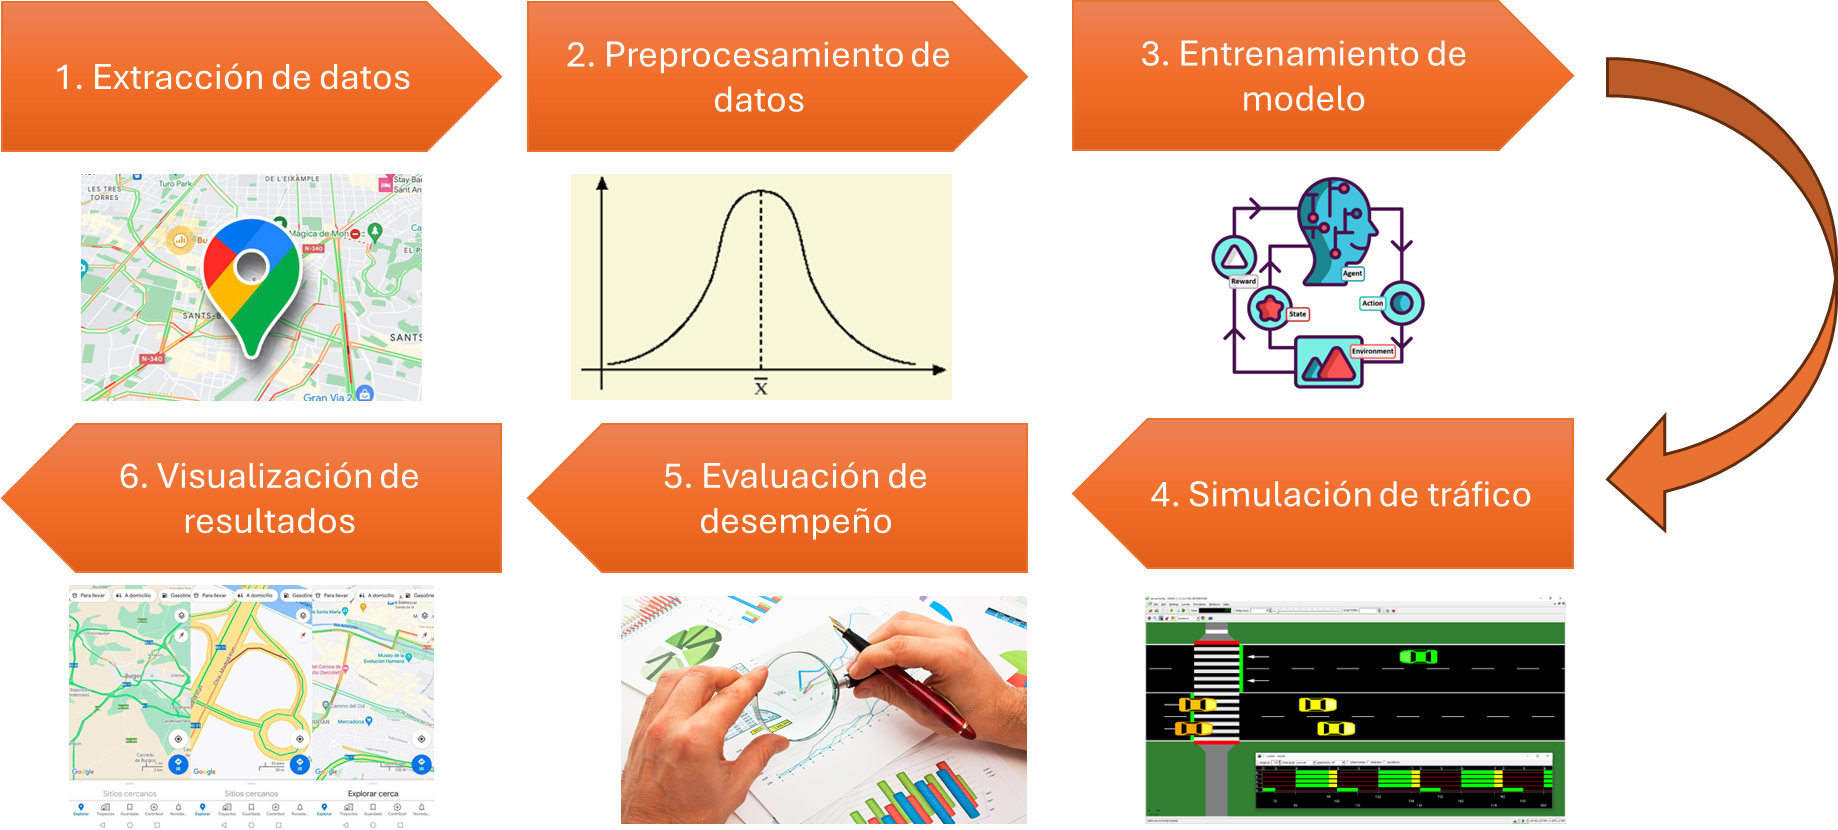
\includegraphics[width=1\linewidth]{metodologia.png}
    \caption{Metodología del proceso}
    \label{metproc}
\end{figure}

\subsection{Extracción de datos}

El primer paso de la metodología consiste en la recopilación de datos históricos y en tiempo real sobre el tráfico vehicular en las intersecciones seleccionadas de la avenida Caminos del Inca. Este proceso garantiza la obtención de información precisa y representativa para el diseño y validación del modelo de aprendizaje por refuerzo.

La recopilación de datos se llevará a cabo mediante APIs de servicios de navegación como Google Maps y Waze, que proporcionan información detallada sobre tiempos de espera, densidad vehicular y velocidades promedio en las intersecciones clave. Estos datos serán recolectados durante un período de observación de cuatro a seis semanas, abarcando tanto horas pico como no pico, para garantizar la representatividad de las diferentes condiciones de tráfico.

Además, se utilizarán herramientas de cartografía en línea como Google Maps Street View y OpenStreetMap para identificar la ubicación exacta de los semáforos en las intersecciones seleccionadas. Esta información será complementada con datos abiertos proporcionados por el municipio de Santiago de Surco, en caso de estar disponibles, para corroborar la existencia y configuración de la infraestructura semafórica.

Finalmente, se llevará a cabo un proceso de validación de los datos recolectados mediante el contraste con informes previos de tráfico y estudios de movilidad realizados en la zona. Esto asegurará que los datos utilizados sean confiables y adecuados para la simulación computacional y el entrenamiento del modelo.

\subsection{Preprocesamiento de datos}

El preprocesamiento de datos es un paso crucial para garantizar la calidad y la usabilidad de la información recolectada. Este proceso tiene como objetivo limpiar, transformar y estructurar los datos recopilados de las APIs y herramientas de navegación para que puedan ser utilizados de manera eficiente en la simulación y el entrenamiento del modelo de aprendizaje por refuerzo.

Inicialmente, los datos serán revisados para detectar inconsistencias, valores atípicos y datos faltantes. Se utilizarán técnicas de interpolación y sustitución para completar los valores ausentes y normalizar las métricas obtenidas, como los tiempos de espera, densidad vehicular y velocidades promedio. Esta normalización garantizará que los datos estén dentro de un rango uniforme, facilitando el entrenamiento del modelo.

Posteriormente, se estructurarán los datos en un formato compatible con el simulador SUMO y los algoritmos de aprendizaje por refuerzo. Esto incluye la conversión de los datos de tráfico en entradas específicas para el modelo, como estados (densidad vehicular en cada dirección), acciones (duración de las fases de semáforo) y recompensas (reducción de tiempos de espera y longitud de colas).

Finalmente, se realizará una segmentación temporal de los datos para analizar patrones de tráfico diferenciados entre horas pico y no pico. Esta segmentación permitirá entrenar el modelo bajo escenarios variados, mejorando su capacidad de generalización y adaptabilidad. Los datos procesados serán almacenados en un repositorio estructurado para su posterior uso en la etapa de simulación y modelado.

\subsection{Entrenamiento de modelo}

El entrenamiento del modelo se lleva a cabo utilizando un marco de aprendizaje por refuerzo profundo (DRL), donde cada semáforo de las intersecciones seleccionadas se representa como un agente independiente. Este agente interactúa con su entorno (condiciones de tráfico) y aprende políticas óptimas a través de un proceso iterativo de prueba y error, con el objetivo de reducir el tiempo de espera promedio y optimizar el flujo vehicular.

Para este proceso, se empleará el simulador SUMO (Simulation of Urban MObility), que permite modelar con precisión las interacciones de los vehículos y la infraestructura semafórica en escenarios urbanos. El entorno de simulación replica las condiciones de tráfico observadas en la avenida Caminos del Inca, integrando los datos procesados previamente. Este simulador proporciona un marco controlado y escalable para probar diversas configuraciones de tráfico.

El modelo se entrenará con un algoritmo de aprendizaje por refuerzo, como el Deep Q-Network (DQN), que utiliza una red neuronal profunda para aproximar las recompensas esperadas de cada acción posible. Estas acciones incluyen cambios en la duración de las fases de luz verde, amarilla y roja en cada semáforo. El entrenamiento se ejecutará en iteraciones múltiples, cada una representando un episodio en el simulador, donde el agente observa el estado del tráfico, toma decisiones y ajusta sus políticas basándose en la retroalimentación obtenida.

Durante el proceso de entrenamiento, se empleará un enfoque multiagente, permitiendo que los semáforos colaboren y compartan información para optimizar el rendimiento global del sistema de tráfico. Además, se monitorearán métricas clave como la velocidad promedio de convergencia, el tiempo de espera y la longitud de las colas vehiculares, ajustando los hiperparámetros del modelo (como la tasa de aprendizaje y el factor de descuento) para maximizar su eficiencia.

El resultado de esta etapa será un modelo entrenado capaz de operar en condiciones reales o simuladas, adaptándose dinámicamente a las variaciones del tráfico y mejorando los indicadores clave de desempeño definidos en el estudio.

\subsection{Simulación de tráfico}

La etapa de simulación de tráfico es fundamental para validar el modelo entrenado y analizar su desempeño en escenarios controlados que replican las condiciones reales de la avenida Caminos del Inca. Esta etapa se lleva a cabo utilizando el simulador SUMO (Simulation of Urban MObility), el cual permite modelar redes de tráfico urbanas con alto grado de precisión y flexibilidad.

La simulación se inicia configurando el entorno con los datos procesados previamente, incluyendo las características específicas de las intersecciones seleccionadas, como el número de carriles, las direcciones del flujo vehicular y los patrones observados en horarios pico y no pico. Asimismo, se introducen escenarios variables, como fluctuaciones en la densidad vehicular y eventos aleatorios que puedan alterar el tráfico, para evaluar la capacidad de adaptación del modelo.

El proceso de simulación se repite en múltiples episodios para obtener resultados estadísticamente significativos. Cada iteración permite ajustar los parámetros del modelo y evaluar su estabilidad y rendimiento bajo condiciones diversas. Al finalizar la simulación, se compararán los resultados obtenidos con el sistema tradicional de control fijo de semáforos, estableciendo diferencias en términos de eficiencia y reducción de congestión vehicular.

El uso de herramientas de visualización integradas en SUMO facilita la representación gráfica de los patrones de tráfico antes y después de la implementación del modelo. Estas visualizaciones son esenciales para interpretar los resultados y comunicar de manera efectiva el impacto del sistema propuesto.

\subsection{Evaluación de desempeño}

La etapa de evaluación del modelo tiene como objetivo medir el impacto del sistema de gestión inteligente de semáforos en la mejora del tráfico vehicular en las intersecciones seleccionadas. Este análisis se realiza utilizando métricas clave, las cuales permiten cuantificar la efectividad del modelo propuesto frente al sistema tradicional de control fijo.

Las métricas utilizadas son:
\begin{itemize}
    \item Tiempo promedio de espera por vehículo: Evalúa la reducción del tiempo que los vehículos permanecen detenidos en las intersecciones. Una disminución significativa en esta métrica indica una mejora en la eficiencia del flujo vehicular.
    \item Longitud promedio de las colas: Mide el nivel de congestión en las intersecciones. Esta métrica es crucial para identificar la capacidad del modelo para descongestionar puntos críticos del tráfico.
    \item Volumen vehicular procesado: Determina la cantidad de vehículos que el sistema puede gestionar en un período específico. Este indicador es esencial para evaluar la capacidad de las intersecciones bajo diferentes niveles de demanda vehicular.
\end{itemize}

La evaluación se llevará a cabo en tres etapas principales:

\begin{itemize}
    \item Comparación directa con el sistema tradicional: Se realizarán simulaciones bajo las mismas condiciones de tráfico utilizando tanto el modelo inteligente como el sistema de control fijo. Las diferencias en las métricas clave permiten cuantificar la mejora lograda.
    \item Análisis de escenarios extremos: Se evaluará el desempeño del modelo en condiciones de alta demanda vehicular (horas pico) y bajo tráfico (horas no pico). Esto asegurará que el modelo sea robusto y adaptable a diferentes contextos.
    \item Estadísticas de rendimiento agregado: Los resultados de múltiples simulaciones se promediarán para obtener valores representativos de cada métrica. Se emplean herramientas estadísticas para validar la significancia de las mejoras observadas.
\end{itemize}

\subsection{Visualización de resultados}

La visualización de resultados es una etapa clave en la metodología, ya que permite interpretar de manera clara y comprensible el impacto del modelo de gestión inteligente de semáforos sobre el tráfico vehicular. Para ello, se generarán gráficos comparativos y representaciones visuales que muestren el comportamiento del tráfico antes y después de la implementación del modelo propuesto.

Se elaborarán gráficos de barras y líneas que representen las métricas clave, como el tiempo promedio de espera, longitud de las colas y volumen vehicular procesado. Estos gráficos permitirán observar visualmente las mejoras en el flujo de tráfico bajo el nuevo sistema frente al sistema tradicional de semáforos. Por ejemplo, un gráfico de barras podría mostrar la comparación de los tiempos de espera en las intersecciones durante las horas pico antes y después de la implementación del modelo de aprendizaje por refuerzo, destacando la reducción en los tiempos de espera promedio.

Se utilizarán diagramas de dispersión y mapas de calor para visualizar la distribución del tráfico a lo largo de la avenida en diferentes horarios del día. Estos mapas facilitarán la identificación de puntos críticos y mostrarán cómo la distribución del tráfico cambia con el ajuste dinámico de los semáforos. Además, los mapas de flujo vehicular podrán ilustrar el impacto en la fluidez del tráfico en intersecciones claves, destacando las áreas con mejoras significativas en la capacidad de procesamiento de vehículos.

A través de gráficos de líneas y áreas, se podrán representar las variaciones en la longitud de las colas en tiempo real, lo que permitirá observar cómo el modelo responde a fluctuaciones en la densidad vehicular. Este tipo de visualización es crucial para entender la efectividad del sistema en escenarios de congestión extrema y su capacidad para reducir los cuellos de botella en las intersecciones.

Se desarrollarán gráficos de series temporales que muestren la evolución de los tiempos de espera y la fluidez vehicular durante las horas pico y no pico. Esto ayudará a resaltar las diferencias en el rendimiento del sistema durante diferentes períodos del día y evaluar la adaptabilidad del modelo a las variaciones en la demanda del tráfico.

Estos gráficos y representaciones serán herramientas clave no solo para la interpretación interna de los resultados, sino también para la presentación de los hallazgos a los tomadores de decisiones y otros interesados, facilitando la justificación de la efectividad del sistema propuesto.

\section{Cronograma y presupuesto}

En esta sección se observa el cronograma cumplido para el desarrollo de la primera parte de la presente tesis.

\begin{figure}[H]
    \centering
    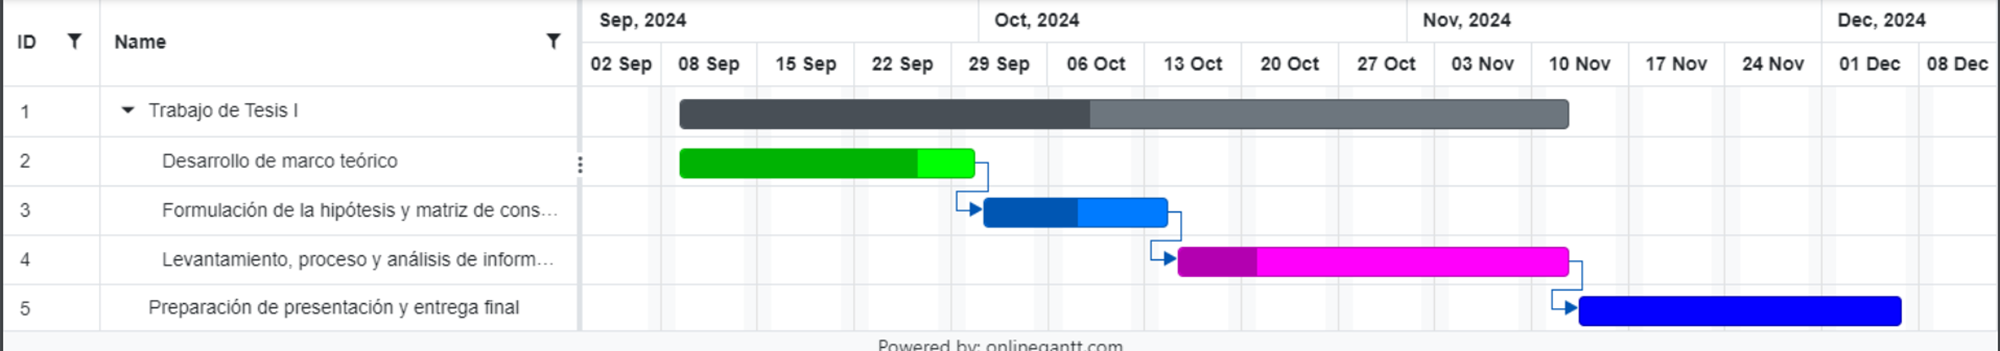
\includegraphics[width=1\linewidth]{gantt.png}
    \caption{Cronograma de primera parte}
    \label{fig:enter-label}
\end{figure}

Por otro lado, se presenta el presupuesto con los principales gastos asociados al desarrollo del modelo.

\begin{table}[H]
	\caption[Presupuesto]{Presupuesto de la investigación.}
	\label{3:table1}
	\centering
	\small
	\begin{tabular}{llll}
		\specialrule{.1em}{.05em}{.05em}
		{Grupo} & {Item} & {Costo (soles)} & {Subtotal} \\
		\specialrule{.1em}{.05em}{.05em}
	{Recursos} & {Equipo de cómputo} & {S/ 3,000.00} & {S/ 3,000.00} \\
		\cline{1-4}
        {Software} & {Simulador} & {S/ 100.00} & {} \\
		{} & {Mantenimiento de equipo} & {S/ 300.00} & {S/ 400.00} \\ % & {S/ 5,274.15} \\
		\cline{1-4}
		\multirow{2}{4cm}

	\end{tabular}
	\begin{flushleft}	
		\small Fuente: Elaboración propia.
	\end{flushleft}
\end{table}




%\include{4/desarrollo}
%\include{5/resultados}
%\include{6/conclusion}

%%Para insertar los capítulos de forma seguida
\chapter{Planteamiento del Problema}
\section{Descripción de la Realidad Problemática}
En el distrito de Santiago de Surco, Lima, la congestión vehicular es un desafío crítico que impacta negativamente tanto en la calidad de vida de sus habitantes como en el desarrollo económico del área. Este problema se agrava por la ineficiencia en la gestión del tráfico, una situación que refleja una falta de adaptación tecnológica para responder a los crecientes retos urbanos. La congestión vehicular en Surco no solo prolonga los tiempos de viaje, sino que también incrementa los costos operativos y el consumo de combustible, lo que a su vez contribuye a la contaminación ambiental. Según un estudio, el tráfico en Lima es uno de los más caóticos de América Latina, con tiempos de viaje que frecuentemente superan el 60\% de lo estimado en condiciones normales, impactando gravemente la productividad y la economía de los hogares, según \cite{swarco2024}. En Surco, un distrito caracterizado por su heterogeneidad socioeconómica y su densa infraestructura urbana, estas condiciones son particularmente críticas debido a su creciente parque automotor, según \cite{sabogal2019}.

Actualmente, los semáforos en las principales intersecciones de Surco operan con ciclos predefinidos, independientemente del flujo real de vehículos. Este sistema rígido genera largas esperas en horas pico y un uso ineficiente del tiempo durante períodos de baja circulación, según \cite{wagner2024}. Además, la ausencia de una infraestructura tecnológica avanzada limita la capacidad del distrito para implementar soluciones dinámicas que mejoren la sincronización de los semáforos y respondan a situaciones inesperadas, como accidentes o bloqueos, según \cite{sabogal2019}.

El tiempo adicional que los vehículos permanecen detenidos aumenta las emisiones de gases contaminantes, lo que afecta la calidad del aire y la salud pública. La Organización Mundial de la Salud ha señalado que la contaminación del aire en ciudades como Lima contribuye significativamente a enfermedades respiratorias y cardiovasculares, un problema especialmente preocupante en zonas densamente urbanizadas como Surco, según \cite{swarco2024}. Socialmente, los embotellamientos generan estrés en los conductores y afectan la convivencia urbana, exacerbando los riesgos de accidentes viales, según \cite{wagner2024}.

En este contexto, la implementación de un sistema de gestión inteligente de semáforos basado en aprendizaje por refuerzo ofrece una solución prometedora. Este enfoque permite que los semáforos ajusten dinámicamente los tiempos de luz verde y roja en función de las condiciones del tráfico en tiempo real, mejorando significativamente el flujo vehicular y reduciendo los tiempos de espera, según \cite{swarco2024}. Además, tecnologías como la inteligencia artificial y los sistemas de modelado de tráfico pueden facilitar la toma de decisiones más efectivas para gestionar recursos limitados, como el espacio vial y la capacidad de las intersecciones, según \cite{sabogal2019}.

La congestión vehicular en Surco no es solo un problema de movilidad; también tiene profundas implicaciones económicas, ambientales y sociales. La implementación de un sistema de semáforos inteligentes contribuiría no solo a una mayor eficiencia en el tráfico, sino también a mejorar la calidad de vida de los habitantes del distrito. Este estudio busca ofrecer un modelo replicable para otras ciudades enfrentando problemas similares, contribuyendo a la sostenibilidad urbana y a un futuro más eficiente y equitativo, según \cite{wagner2024}.

\section{Formulación del Problema}

\subsection{Problema General}
PG: \newcommand{\ProblemaGeneral}{
¿Cómo puede un modelo de aprendizaje por refuerzo optimizar la sincronización de los semáforos en Santiago de Surco para mejorar el flujo vehicular y reducir los tiempos de espera en las intersecciones principales y auxiliares?
}
\ProblemaGeneral
\subsection{Problemas Específicos}
\newcommand{\Pbone}{
¿Cómo afecta la falta de un modelo dinámico de aprendizaje por refuerzo a la optimización de los tiempos de los ciclos de luz verde y roja en las intersecciones principales?
}
\newcommand{\Pbtwo}{
¿Qué tan eficaz puede ser el uso de un modelo de aprendizaje por refuerzo para reducir los tiempos de espera en las intersecciones principales de Santiago de Surco durante diferentes franjas horarias?
}
\newcommand{\Pbthree}{
¿Cómo podría un modelo de aprendizaje por refuerzo sincronizar de manera eficiente los semáforos de las vías principales con sus auxiliares para mejorar el flujo vehicular?
}
\newcommand{\Pbfour}{
¿Qué resultados pueden observarse al aplicar un modelo de aprendizaje por refuerzo en las intersecciones seleccionadas, en comparación con los sistemas de semáforos tradicionales?
}

\begin{itemize}
	\item PE1: {\Pbone}
	\item PE2: {\Pbtwo}
	\item PE3: {\Pbthree}
	\item PE4: {\Pbfour}
\end{itemize}

\section{Objetivos de la Investigación}

\subsection{Objetivo General}
OG: \newcommand{\ObjetivoGeneral}{
Diseñar un modelo de aprendizaje por refuerzo para optimizar la sincronización de los semáforos en Santiago de Surco, con el fin de mejorar el flujo vehicular y reducir los tiempos de espera en las intersecciones principales y sus auxiliares.
}
\ObjetivoGeneral
\subsection{Objetivos Específicos}
\newcommand{\Objone}{
Proponer un modelo basado en aprendizaje por refuerzo que permita ajustar dinámicamente los tiempos de luz verde y roja de los semáforos en función de las condiciones del tráfico vehicular.

}
\newcommand{\Objtwo}{
Implementar simulaciones del modelo en escenarios representativos de las intersecciones seleccionadas de Santiago de Surco para evaluar su desempeño frente a los sistemas tradicionales.
}
\newcommand{\Objthree}{

Analizar el impacto del modelo en la reducción de los tiempos de espera en las intersecciones principales y en el flujo vehicular en las vías auxiliares conectadas.
}
\newcommand{\Objfour}{

Validar la efectividad del modelo comparando métricas de tráfico, como tiempo promedio de espera y volumen vehicular procesado, antes y después de su aplicación en simulaciones.
}

\begin{itemize}
	\item OE1: {\Objone}
	\item OE2: {\Objtwo}
	\item OE3: {\Objthree}
	\item OE4: {\Objfour}
\end{itemize}


\section{Hipótesis de la Investigación}
\subsection{Hipótesis General}
HG: \newcommand{\HipotesisGeneral}{
La implementación de un modelo de aprendizaje por refuerzo para la sincronización de semáforos en Santiago de Surco permitirá mejorar el flujo vehicular y reducir significativamente los tiempos de espera en las intersecciones principales y sus auxiliares.
}
\HipotesisGeneral


\subsection{Hipótesis Específicas}
\newcommand{\Hone}{
Un modelo basado en aprendizaje por refuerzo ajustará dinámicamente los tiempos de luz verde y roja, logrando una reducción significativa en los tiempos de espera en las intersecciones principales.

}
\newcommand{\Htwo}{
La sincronización de los semáforos mediante un modelo de aprendizaje por refuerzo mejorará la fluidez vehicular entre las vías principales y sus auxiliares, reduciendo los cuellos de botella en el tráfico.
}
\newcommand{\Hthree}{
La implementación del modelo permitirá procesar un mayor volumen vehicular por intersección en comparación con los sistemas tradicionales de semaforización.
}
\newcommand{\Hfour}{
El uso de un modelo de aprendizaje por refuerzo demostrará, en simulaciones, una mejora notable en las métricas de tráfico, como la reducción de tiempos promedio de espera y el incremento de la eficiencia en la gestión del flujo vehicular.
}

\begin{itemize}
	\item HE1: {\Hone}
	\item HE2: {\Htwo}
	\item HE3: {\Hthree}
	\item HE4: {\Hfour}
\end{itemize}

\section{Justificación de la Investigación}

\subsection{Teórica}
La justificación teórica de esta investigación se fundamenta en el uso del aprendizaje por refuerzo, una técnica de inteligencia artificial que permite a un agente aprender a tomar decisiones optimizadas en un entorno dinámico. Aplicado a la gestión de semáforos, el aprendizaje por refuerzo puede modelar el sistema como un proceso de toma de decisiones secuenciales, donde cada semáforo actúa como un agente autónomo que mejora su desempeño a través de la experiencia. Esta teoría de control adaptativo permite implementar sistemas que se ajustan a las condiciones cambiantes del tráfico, promoviendo una mayor eficiencia en la gestión vehicular.

\subsection{Práctica}
La justificación práctica se basa en la necesidad urgente de optimizar la gestión del tráfico en Santiago de Surco, un distrito con intersecciones congestionadas debido a semáforos mal sincronizados. Al implementar un sistema inteligente basado en aprendizaje por refuerzo, los semáforos podrán adaptarse a las condiciones reales del tráfico, reduciendo los tiempos de espera y mejorando la fluidez vehicular. Esto no solo beneficiará a los conductores, sino también al transporte público y a los peatones, al disminuir los tiempos de viaje, el consumo de combustible y la emisión de gases contaminantes.

\subsection{Metodológica}
La justificación metodológica de esta investigación radica en la aplicación de técnicas de simulación y modelado para probar la eficacia del aprendizaje por refuerzo en la gestión de semáforos. Se utilizarán herramientas de simulación de tráfico para replicar las condiciones reales de las intersecciones de Santiago de Surco, permitiendo evaluar el rendimiento del sistema propuesto. Este enfoque experimental permitirá ajustar los parámetros del modelo en un entorno controlado antes de su implementación en el mundo real, garantizando una mayor precisión en los resultados y reduciendo los riesgos asociados a la puesta en marcha del sistema.
\section{Delimitación del Estudio}

\subsection{Espacial}
El estudio se llevará a cabo en el municipio de Santiago de Surco, uno de los distritos más grandes y transitados de Lima, Perú. El área de enfoque principal será las intersecciones vehiculares más congestionadas, donde el tráfico es más caótico y la sincronización de los semáforos es crucial para mejorar la fluidez. El proyecto se centrará en áreas clave, como avenidas principales y cruces donde la congestión vehicular es frecuente. Estas zonas han sido seleccionadas debido a su alta densidad vehicular y la necesidad evidente de mejorar la gestión del tráfico.

\subsection{Temporal}
El proyecto tomará métricas del tráfico durante el año 2024. El proyecto incluirá desde la planificación y el diseño del sistema hasta la evaluación final de su efectividad mediante simulaciones de tráfico. El estudio incluye la recolección de datos actuales sobre el tráfico en las intersecciones seleccionadas, la creación del modelo de aprendizaje por refuerzo, y la prueba del sistema en un entorno simulado. El tiempo estimado, de 1 año, es suficiente para realizar ajustes en el modelo y evaluar su desempeño en diferentes escenarios, asegurando que el sistema funcione de manera óptima antes de su posible implementación.

\subsection{Conceptual}
El estudio se centrará en el diseño e implementación de un sistema de gestión inteligente de semáforos basado en el aprendizaje por refuerzo. Este sistema busca mejorar la sincronización y la gestión del tráfico vehicular en las intersecciones seleccionadas de Santiago de Surco. El aprendizaje por refuerzo se entiende como una técnica de inteligencia artificial que permite a los agentes, en este caso los semáforos, tomar decisiones óptimas a través de la interacción con su entorno. El sistema busca optimizar el flujo vehicular, reducir tiempos de espera y mejorar la eficiencia general del tránsito urbano.


\chapter{Marco Teórico}
\section{Antecedentes de la investigación}
El artículo de \cite{Joo2020} titulado "Traffic Signal Control for Smart Cities Using Reinforcement Learning" propone un sistema de control de señales de tráfico basado en aprendizaje por refuerzo, específicamente utilizando el algoritmo Q-learning (QL), para mejorar la gestión del tráfico en intersecciones dentro del contexto de ciudades inteligentes.

El problema principal abordado es la incapacidad de los sistemas tradicionales de control de tráfico con tiempos fijos para adaptarse a entornos dinámicos y datos complejos generados por las ciudades inteligentes. Estas limitaciones resultan en congestión, mayores tiempos de espera y un desequilibrio en la distribución de señales de tráfico, lo que afecta la eficiencia y equidad del sistema.

La metodología incluye la formulación de un modelo que utiliza Q-learning con un enfoque en el rendimiento (throughput) y la desviación estándar de las longitudes de cola como parámetros principales. Se diseñó un entorno simulado con SUMO para representar una intersección de cuatro vías, donde se evaluó el sistema mediante métricas de longitud de cola, desviación estándar de las colas y tiempos de espera promedio. Los estados se definieron en función del flujo vehicular por dirección, mientras que las recompensas se calcularon combinando la desviación estándar de las colas y el rendimiento mediante una función adaptativa.

Los resultados experimentales muestran que el algoritmo propuesto supera a modelos previos de Q-learning en todas las métricas evaluadas. En comparación con un modelo basado en tiempos fijos mejorado (E-TS) y un modelo basado en clústeres (C-TS), el sistema propuesto redujo la longitud de cola promedio en un 25\% frente a E-TS y un 63\% frente a C-TS. Además, disminuyó la desviación estándar de las colas en un 50\% y 75\%, respectivamente. En términos de tiempo de espera promedio por vehículo, el sistema logró una reducción del 15\% frente a E-TS y del 40\% frente a C-TS.

Estos resultados confirman que el sistema propuesto no solo es efectivo en reducir los tiempos de espera y equilibrar las señales, sino que también es escalable a diferentes configuraciones de intersecciones, mostrando potencial para implementaciones prácticas en ciudades inteligentes.

\cite{Li2021} presenta el artículo "Network-wide Traffic Signal Control Optimization Using a Multi-agent Deep Reinforcement Learning", donde se explora la problemática de la congestión vehicular en redes complejas de intersecciones múltiples, analizando cómo los enfoques tradicionales de control de tráfico, como los sistemas de tiempos fijos o descentralizados, no logran adaptarse dinámicamente a las condiciones cambiantes del tráfico. Estos métodos resultan en mayores tiempos de espera, congestión severa y un desperdicio significativo de recursos energéticos. El trabajo destaca la necesidad de enfoques más inteligentes y colaborativos para optimizar el control de señales de tráfico en redes urbanas extensas.

La metodología se centra en el desarrollo de un sistema basado en aprendizaje por refuerzo profundo multi-agente (KS-DDPG), que combina un aprendizaje centralizado con una ejecución descentralizada. Este sistema permite a los agentes en cada intersección tomar decisiones dinámicas basadas en un protocolo de compartición de conocimiento entre agentes. Las simulaciones del sistema se llevaron a cabo utilizando el simulador de tráfico SUMO, además de datos reales extraídos de redes de tráfico en Montgomery County, Maryland. Los indicadores clave de rendimiento incluyeron la longitud promedio de colas y el tiempo promedio de retraso por vehículo.

El modelo KS-DDPG integra un mecanismo de comunicación que permite a los agentes compartir experiencias relevantes y aprender colectivamente. Este enfoque colaborativo mejora significativamente la capacidad de los agentes para tomar decisiones óptimas sobre la duración de las fases de los semáforos, logrando así una sincronización eficiente en condiciones de tráfico fluctuantes. La arquitectura del modelo garantiza que el sistema sea escalable y eficiente, adaptándose a redes de tráfico complejas.

Los resultados del estudio demostraron que el modelo KS-DDPG supera ampliamente a otros métodos, como los sistemas de aprendizaje por refuerzo tradicional (DQN y MADDPG), y a los métodos de control de tráfico convencionales. Redujo notablemente la longitud de las colas y los tiempos de retraso, especialmente en escenarios de alta demanda vehicular, destacándose como una solución robusta para optimizar el flujo de tráfico en entornos urbanos.

El artículo de \cite{Li2021a} titulado "A Deep Reinforcement Learning Approach for Traffic Signal Control Optimization" aborda el desafío de optimizar las señales de tráfico en redes urbanas complejas utilizando un enfoque avanzado de aprendizaje por refuerzo profundo (DRL). El problema principal identificado es la ineficiencia de los sistemas de semaforización tradicionales y adaptativos, los cuales a menudo generan largos tiempos de espera y mayor congestión debido a su incapacidad para adaptarse dinámicamente a las condiciones fluctuantes del tráfico en tiempo real. Este trabajo introduce el algoritmo MADDPG (Multi-Agent Deep Deterministic Policy Gradient) como solución a estas limitaciones, combinando aprendizaje centralizado y ejecución descentralizada para abordar los retos de escalabilidad y coordinación en redes con múltiples intersecciones.

La metodología empleada se centra en un marco de Aprendizaje por Refuerzo Multiagente, modelando cada semáforo como un agente independiente en un entorno cooperativo-competitivo. Los datos del tráfico, como la longitud de las colas y el tiempo de espera, se obtienen mediante detectores en bucle y simulaciones con el software SUMO. Los agentes ajustan dinámicamente las fases de los semáforos basándose en observaciones locales y recompensas diseñadas para minimizar las demoras y optimizar el flujo vehicular. Durante el entrenamiento, el modelo utiliza una combinación de redes neuronales profundas (actor y crítico) para aprender políticas óptimas de control.

Los resultados del experimento, evaluados en un entorno de simulación que replica la red de tráfico del condado de Montgomery, Maryland, destacan la eficacia del algoritmo MADDPG en comparación con otros métodos como DQN y DDPG. En métricas clave como la longitud promedio de colas y el tiempo de espera por vehículo, MADDPG mostró una reducción significativa frente a los controladores de tiempo fijo y otros enfoques basados en DRL. Además, el sistema logró una mayor estabilidad en sus políticas de control, superando los problemas de no estacionariedad y alta varianza que suelen afectar a otros métodos.

El estudio concluye que MADDPG es una herramienta robusta y escalable para el control adaptativo de señales de tráfico en redes complejas. Sin embargo, también señala limitaciones relacionadas con la representación de estados en espacios de alta dimensionalidad y la necesidad de mejorar la eficiencia del aprendizaje en escenarios de datos limitados. Estos resultados refuerzan el potencial del aprendizaje por refuerzo profundo como una solución viable para los sistemas inteligentes de transporte en entornos urbanos.

El artículo de \cite{Mo2022} titulado "CVLight: Decentralized learning for adaptive traffic signal control with connected vehicles" presenta una metodología para optimizar el control de señales de tráfico en múltiples intersecciones mediante un esquema descentralizado de aprendizaje por refuerzo (RL), denominado CVLight. El principal problema que aborda este estudio es la dificultad de aplicar métodos tradicionales de control de semáforos a redes de tráfico dinámicas, donde los vehículos conectados (CV) pueden proporcionar información detallada y en tiempo real sobre el flujo vehicular. Sin embargo, los sistemas de control clásicos no logran aprovechar estos datos de manera eficiente, especialmente cuando la penetración de vehículos conectados es baja, lo que puede generar una optimización subóptima del flujo vehicular.

La metodología empleada en el artículo es un enfoque de aprendizaje por refuerzo descentralizado, utilizando un algoritmo novedoso llamado Asymmetric Advantage Actor-Critic (Asym-A2C), que emplea información parcial de los vehículos conectados (CVs) para entrenar el "actor" y la información completa (de CVs y vehículos no conectados) para entrenar el "crítico". En este esquema, los agentes (semáforos) se entrenan para seleccionar fases de semáforo de forma autónoma basándose en las observaciones que hacen de los vehículos presentes en cada intersección. Este enfoque permite que el sistema se adapte a situaciones de tráfico variadas, optimizando la duración de las fases de semáforo y reduciendo los retrasos en las intersecciones, incluso en escenarios con baja penetración de vehículos conectados.

Los experimentos realizados en el artículo utilizan una red de intersecciones de tamaño 2x2, con simulaciones que reflejan condiciones de tráfico dinámicas y variaciones en la tasa de penetración de CVs. Los resultados muestran que CVLight supera a los métodos tradicionales de control de semáforos y otros enfoques de aprendizaje por refuerzo, mostrando mejoras significativas en el tiempo de espera promedio por vehículo y en la eficiencia del tráfico. Específicamente, el modelo mostró una reducción del 30\% en el tiempo de espera promedio por vehículo con una penetración de CVs del 20\%, comparado con los modelos tradicionales. También se evaluó la escalabilidad del sistema, demostrando que el enfoque de preentrenamiento del modelo permite aplicar CVLight a redes de tráfico más grandes, como un sistema 5x5, con costos computacionales reducidos.

Los resultados de estos experimentos resaltan que el sistema CVLight no solo es efectivo en escenarios de alta penetración de CVs, sino que también ofrece una solución robusta cuando la penetración de CVs es baja, lo que lo convierte en una opción viable para el futuro de los sistemas de gestión del tráfico inteligente. Además, se destaca que el uso de un algoritmo de aprendizaje por refuerzo descentralizado permite que cada intersección aprenda de manera independiente, promoviendo la cooperación entre las intersecciones sin la necesidad de un sistema de control centralizado.

El artículo de \cite{Damadam2022} titulado "An Intelligent IoT Based Traffic Light Management System: Deep Reinforcement Learning" presenta un enfoque para el control adaptativo de señales de tráfico utilizando aprendizaje por refuerzo profundo y tecnologías IoT, aplicado en seis intersecciones de la ciudad de Shiraz, Irán.

El principal problema que aborda el artículo es la ineficiencia de los sistemas de control de tráfico basados en tiempos fijos, que no pueden adaptarse a las condiciones dinámicas del tráfico, lo que genera congestión, mayor consumo de combustible y contaminación ambiental. Además, estos sistemas presentan costos elevados de implementación y mantenimiento, lo que limita su viabilidad en ciudades metropolitanas.

La metodología incluye la implementación de un algoritmo de Aprendizaje por Refuerzo Multi-Agente (MARL, por sus siglas en inglés) combinado con el algoritmo Advantage Actor-Critic (A2C). Este sistema descentralizado utiliza sensores IoT como cámaras de vigilancia para recopilar datos de tráfico en tiempo real, como las longitudes de cola y los tiempos de espera de los vehículos, que son procesados localmente y compartidos entre agentes para optimizar las señales de tráfico. Además, se incorpora el método de huellas dactilares para estabilizar el aprendizaje entre agentes.

En términos de evaluación, los experimentos fueron realizados en un simulador de tráfico urbano (SUMO) utilizando datos reales de tráfico proporcionados por el municipio de Shiraz. Los resultados numéricos muestran una mejora significativa en la gestión del tráfico en comparación con el sistema de tiempos fijos existente. En promedio, el sistema propuesto logró reducir las longitudes de cola en un 20-30\% y los tiempos de espera de los vehículos en un 25\% en las seis intersecciones estudiadas.

Estos resultados destacan el potencial del uso combinado de técnicas de aprendizaje por refuerzo profundo y tecnologías IoT para mejorar la eficiencia del tráfico urbano, promoviendo un sistema de control robusto y escalable.

El artículo de \cite{Cao2024} titulado "Optimization Control of Adaptive Traffic Signal with Deep Reinforcement Learning" propone una metodología para optimizar el control adaptativo de señales de tráfico utilizando un algoritmo mejorado basado en aprendizaje por refuerzo profundo denominado G-DQN, implementado y evaluado mediante simulaciones en el software SUMO.

El problema principal identificado es la ineficacia de los esquemas tradicionales de control de tráfico con tiempos fijos, que no pueden adaptarse a las condiciones de tráfico dinámico. Esto resulta en mayores tiempos de espera, congestión, y una gestión subóptima del tráfico en intersecciones complejas. Adicionalmente, las estrategias de aprendizaje por refuerzo existentes presentan limitaciones en la representación de estados y recompensas, así como en la convergencia eficiente de los modelos.

La metodología se basa en el desarrollo del algoritmo G-DQN, que introduce mejoras en la estructura de redes neuronales convolucionales (CNN) para procesar matrices duales de estado (posición y velocidad de vehículos), y redefine los estados y recompensas para reflejar con mayor precisión las condiciones de tráfico. También utiliza un enfoque dinámico para la selección de acciones con el método e-greedy y simula datos de tráfico usando la distribución Weibull para emular patrones de tráfico reales.

En los experimentos, se compararon los resultados del G-DQN con el algoritmo DQN original, el algoritmo A2C y un esquema de tiempo fijo. Los resultados numéricos muestran que el G-DQN redujo el tiempo acumulado en cola a 26,676 segundos, frente a 38,870 del DQN y 40,538 del esquema fijo, el promedio de longitud de cola fue de 4.9 vehículos para el G-DQN, comparado con 7.2 del DQN y 8.0 del esquema fijo, y el G-DQN logró la convergencia en 3200 pasos, más rápido que el DQN (4100 pasos) y comparable al A2C (3600 pasos).

Estos resultados demuestran que el G-DQN mejora significativamente la eficiencia del tráfico en intersecciones simuladas, optimizando tanto el tiempo de espera como la longitud de las colas en comparación con los métodos tradicionales y otros enfoques de aprendizaje por refuerzo.

El artículo de \cite{Gu2021} titulado "Traffic Signal Optimization for Multiple Intersections Based on Reinforcement Learning" propone un modelo de optimización de señales de tráfico basado en aprendizaje por refuerzo profundo, diseñado para operar bajo restricciones reales de intersecciones múltiples. El modelo mantiene la secuencia típica de fases de semáforo y considera un tiempo mínimo de luz verde, aspectos clave para su aplicabilidad en entornos reales.

El problema principal abordado en el estudio es la limitación de los modelos tradicionales de control de señales fijas y de algunos modelos de aprendizaje por refuerzo existentes, que a menudo ignoran restricciones operativas como la secuencia fija de fases y el tiempo mínimo de luz verde. Estos enfoques pueden resultar en configuraciones no viables, causando confusión entre los conductores y vehículos con tiempos de espera excesivos.

La metodología se centra en un modelo basado en Deep Q-Network (DQN), entrenado en un entorno simulado con SUMO (Simulation of Urban MObility). Los estados del modelo incluyen la cola de vehículos por carril, la fase activa del semáforo y el tiempo transcurrido de la fase activa. Las acciones posibles son mantener la fase actual o cambiar a la siguiente, siempre respetando las restricciones de tiempo mínimo verde y secuencia de fases. La recompensa se define como el cociente entre los vehículos que pasan y los detenidos durante un intervalo de tiempo.

En los experimentos realizados, se evaluaron dos escenarios. En el primero, con dos intersecciones conectadas, el modelo propuesto redujo el retraso promedio por vehículo de 40 segundos a 30 segundos y el número promedio de paradas de 2.5 a 2, comparado con un modelo fijo. En el segundo escenario, que incluye seis intersecciones en una red realista, se obtuvo una reducción del 88\% al 31\% en el retraso acumulado y del 95\% al 46\% en el número de paradas acumuladas frente al modelo fijo. Durante las horas pico, el retraso promedio se redujo de 3 minutos y 15 segundos a 2 minutos y 15 segundos, mientras que el número de paradas promedio por vehículo disminuyó de 11 a 4.7.

Estos resultados destacan que, aunque el modelo propuesto no supera en todas las métricas a un modelo de comparación sin restricciones, ofrece una solución más realista y aplicable para su implementación en el mundo real, asegurando un equilibrio entre eficiencia y viabilidad práctica.

El artículo de \cite{Rasheed2020} titulado "Deep Reinforcement Learning for Traffic Signal Control: A Review" presenta una revisión exhaustiva sobre el uso del aprendizaje por refuerzo profundo (DRL) para el control de señales de tráfico, abarcando arquitecturas, plataformas de simulación, análisis de complejidad, y métricas de rendimiento.

El principal problema que aborda es la complejidad creciente en la gestión del tráfico urbano debido al aumento de la congestión vehicular, causada por el crecimiento poblacional y la urbanización. Los métodos tradicionales de control de tráfico enfrentan limitaciones como el costo computacional elevado y la incapacidad para adaptarse a entornos dinámicos y no estructurados, especialmente en redes de tráfico densas.

La metodología revisa las arquitecturas más comunes de DRL aplicadas al control de tráfico, incluyendo redes neuronales convolucionales (CNN), redes neuronales totalmente conectadas (FCLN), y redes LSTM, explorando sus capacidades para representar espacios de estado complejos y optimizar señales de tráfico. Además, se analizan las plataformas de simulación, como SUMO y Aimsun, que permiten modelar redes de tráfico realistas y evaluar los algoritmos propuestos.

Los resultados muestran que las soluciones basadas en DRL superan significativamente a los enfoques tradicionales en métricas clave como tiempo promedio de espera, longitud de cola promedio y rendimiento (throughput). Por ejemplo, se reporta que algunas implementaciones logran reducir el tiempo de espera promedio en un 15-30\% en comparación con sistemas de tiempo fijo, dependiendo del escenario de simulación y la arquitectura de DRL utilizada.

El artículo también identifica desafíos abiertos, como la escalabilidad de los modelos para redes de múltiples intersecciones y la integración de datos de tráfico en tiempo real, planteando direcciones futuras de investigación.

El artículo de \cite{Zhu2022} titulado "Traffic Sign Recognition Based on Deep Learning" presenta un análisis comparativo entre los modelos YOLOv5 y SSD para la detección y reconocimiento de señales de tráfico, evaluando su rendimiento en términos de precisión, velocidad y adaptabilidad en un conjunto de datos creado específicamente para este estudio.

El problema principal identificado es la incapacidad de los métodos tradicionales de reconocimiento de señales de tráfico para manejar escenarios complejos en tiempo real, como cambios en la iluminación, ángulos de cámara y oclusiones. Esto limita su aplicabilidad en sistemas de transporte inteligente y vehículos autónomos.

La metodología empleada incluye la recopilación de un conjunto de datos personalizado con 2,182 imágenes de señales de tráfico organizadas en ocho clases. Se implementaron experimentos utilizando YOLOv5 y SSD en la plataforma Google Colab con GPU de alto rendimiento, evaluando los modelos mediante métricas como precisión promedio (mAP) y velocidad de reconocimiento (FPS).

En los resultados, YOLOv5 superó significativamente a SSD en precisión y velocidad. YOLOv5 alcanzó un mAP promedio de 97.70\% para todas las clases, mientras que SSD logró un 90.14\%. En términos de velocidad, YOLOv5 procesó imágenes a 30 FPS, mientras que SSD lo hizo a 3.49 FPS, lo que indica que YOLOv5 es aproximadamente 10 veces más rápido.

El estudio concluye que YOLOv5 es más adecuado para entornos de tráfico en tiempo real debido a su alta precisión y velocidad, destacando su potencial para aplicaciones en sistemas de transporte inteligente.



\section{Bases Teóricas}
\subsection{Gestión del tráfico vehicular}
La gestión del tráfico vehicular es un componente crítico de la planificación urbana, ya que los problemas de congestión no solo afectan los tiempos de viaje, sino que también incrementan el consumo de combustible y las emisiones contaminantes. Los sistemas tradicionales de semaforización, basados en tiempos fijos, presentan limitaciones significativas, ya que no pueden adaptarse a cambios dinámicos en el flujo vehicular. En este contexto, los sistemas adaptativos han surgido como una solución avanzada, utilizando datos en tiempo real para ajustar las fases semafóricas, lo que permite reducir los tiempos de espera y mejorar el flujo vehicular en intersecciones críticas, según \cite{SustainableTraffic2020}.

La gestión del tráfico vehicular no solo implica la regulación del flujo vehicular en las calles, sino que también abarca la implementación de políticas que reduzcan la demanda de transporte motorizado y fomenten alternativas sostenibles, como el uso del transporte público y la movilidad activa. Un enfoque integral en la planificación del tráfico requiere considerar tanto el diseño físico de las ciudades como las dinámicas sociales y económicas que influyen en el comportamiento de los usuarios de las vías. En este sentido, los sistemas adaptativos y la sincronización dinámica de semáforos juegan un papel clave al permitir ajustes en tiempo real basados en datos sobre densidad vehicular y patrones de tráfico.

En particular, el uso de sensores y tecnologías de comunicación permite recopilar datos en tiempo real que alimentan algoritmos avanzados para optimizar las decisiones de control de tráfico. Sensores como cámaras, detectores inductivos y sistemas de posicionamiento global (GPS) pueden proporcionar información detallada sobre el volumen, la velocidad y la dirección del tráfico. Estos datos, procesados mediante modelos predictivos y sistemas inteligentes, pueden generar estrategias para minimizar los tiempos de espera y evitar la formación de cuellos de botella en las intersecciones más congestionadas.

Además, la integración de enfoques de inteligencia artificial en la gestión del tráfico ha revolucionado la capacidad de respuesta de los sistemas de transporte urbano. Por ejemplo, los sistemas adaptativos pueden priorizar ciertas rutas durante emergencias o eventos masivos, ajustando dinámicamente los semáforos para facilitar el paso de vehículos de emergencia o desviar el tráfico de zonas críticas. Esta flexibilidad no solo mejora la eficiencia de las ciudades, sino que también tiene un impacto significativo en la calidad de vida de los ciudadanos al reducir el estrés asociado con el tráfico y promover una movilidad más fluida.

No obstante, la implementación de estos sistemas adaptativos enfrenta desafíos importantes, como el alto costo inicial de las infraestructuras necesarias y la necesidad de una interoperabilidad entre diferentes tecnologías. Además, es fundamental garantizar la seguridad y privacidad de los datos recopilados, así como educar a los usuarios para que comprendan y se adapten a estos sistemas. A pesar de estos retos, las inversiones en gestión avanzada del tráfico han demostrado ser rentables a largo plazo, generando beneficios tanto económicos como medioambientales para las ciudades y sus habitantes.

\subsection{Aprendizaje por refuerzo}
El aprendizaje por refuerzo es una técnica de inteligencia artificial basada en la interacción continua entre un agente y su entorno. El agente aprende políticas óptimas mediante un proceso iterativo de ensayo y error, donde las recompensas obtenidas guían su aprendizaje. Este enfoque es particularmente relevante para sistemas de gestión de tráfico, ya que permite abordar problemas estocásticos y de alta dimensionalidad. Modelos como Q-learning y Deep Q-learning han demostrado ser eficaces en la optimización del tiempo de las señales de tráfico, al adaptarse a condiciones dinámicas y mejorar la eficiencia del sistema, según \cite{ReinforcementLearning2021}.

El aprendizaje por refuerzo (RL, por sus siglas en inglés) se basa en un marco matemático que utiliza la interacción entre un agente y su entorno para aprender a realizar decisiones óptimas a lo largo del tiempo. Este enfoque se fundamenta en conceptos clave como estados, acciones y recompensas. Los estados representan las características observables del entorno en un momento dado, las acciones son las decisiones que el agente puede tomar, y las recompensas son señales de retroalimentación que guían el proceso de aprendizaje. A través de un proceso iterativo, el agente busca maximizar el beneficio acumulado al identificar políticas que relacionen estados con acciones óptimas.

Una característica fundamental del aprendizaje por refuerzo es su capacidad para manejar entornos estocásticos y dinámicos. A diferencia de otros métodos de aprendizaje supervisado, donde se requiere un conjunto de datos etiquetados, el aprendizaje por refuerzo no depende de datos predefinidos, sino que aprende explorando y explotando las posibilidades del entorno. Esta característica lo hace especialmente útil en problemas donde no se conoce a priori la solución óptima o cuando el entorno cambia con el tiempo, como ocurre en la gestión del tráfico vehicular.

El proceso de aprendizaje se estructura comúnmente en términos de un modelo de decisión de Markov (MDP), que proporciona una representación formal del entorno. En este modelo, cada decisión tomada por el agente influye no solo en las recompensas inmediatas, sino también en los estados futuros que determinarán recompensas adicionales. Esto introduce un componente de planificación a largo plazo, ya que el agente debe considerar las consecuencias futuras de sus acciones actuales. Herramientas como Q-learning y Deep Q-learning permiten implementar este enfoque mediante el uso de tablas de valores o redes neuronales profundas que estiman las recompensas esperadas para cada acción posible.

\subsection{Optimización del flujo vehicular}
La optimización del flujo vehicular busca maximizar la movilidad urbana mediante la reducción de tiempos de espera y la minimización de cuellos de botella. Las estrategias incluyen el ajuste dinámico de las fases de los semáforos y la redistribución del tráfico hacia rutas menos congestionadas. Estas técnicas no solo mejoran la experiencia de los usuarios, sino que también contribuyen a la sostenibilidad ambiental al reducir el consumo de combustible y las emisiones de gases contaminantes. Los avances en inteligencia artificial han permitido integrar modelos predictivos que anticipan el comportamiento del tráfico, mejorando la capacidad de respuesta del sistema, según \cite{OptimizingTraffic2019}.

La optimización del flujo vehicular es una disciplina que busca maximizar la eficiencia en el uso de la infraestructura vial, minimizando las demoras, los cuellos de botella y el impacto ambiental asociado al tráfico urbano. Este enfoque teórico parte de la premisa de que el flujo vehicular no es un sistema estático, sino una red dinámica influenciada por variables como la densidad del tráfico, las características de las intersecciones y los patrones de movilidad de los usuarios. A través de modelos matemáticos y simulaciones, se diseñan estrategias para equilibrar las cargas de tráfico y reducir la congestión.

Entre los métodos tradicionales para optimizar el flujo vehicular, destacan los sistemas de control semafórico fijo y las estrategias de programación lineal. Sin embargo, estas técnicas tienen limitaciones significativas, ya que no pueden adaptarse a las condiciones cambiantes del tráfico en tiempo real. Para abordar este problema, se han desarrollado métodos dinámicos que integran herramientas de análisis predictivo y modelos probabilísticos, permitiendo anticipar la formación de cuellos de botella y redistribuir el tráfico hacia rutas menos congestionadas.

Desde una perspectiva teórica, la optimización del flujo vehicular involucra la definición de métricas clave, como el tiempo promedio de espera, la longitud de las colas y la velocidad promedio de los vehículos. Estas métricas se utilizan para evaluar y ajustar las estrategias de control. Por ejemplo, los algoritmos de optimización pueden priorizar ciertas fases semafóricas en función de la densidad vehicular en cada dirección, ajustando dinámicamente la duración de las luces verdes para maximizar la fluidez del tráfico. Este enfoque no solo mejora la experiencia de los conductores, sino que también tiene un impacto positivo en la sostenibilidad ambiental.

\subsection{Modelado y simulación del tráfico}
El modelado y simulación del tráfico son herramientas fundamentales para evaluar soluciones antes de su implementación en escenarios reales. Plataformas como SUMO (Simulation of Urban MObility) y VISSIM ofrecen un entorno controlado para recrear condiciones urbanas complejas. Estas herramientas permiten simular flujos vehiculares, evaluar la efectividad de estrategias de control adaptativo y ajustar modelos teóricos a partir de datos reales. La simulación también facilita la prueba de algoritmos de inteligencia artificial, reduciendo los costos y riesgos asociados con las implementaciones físicas, según \cite{TrafficSimulation2020}.

El modelado y simulación del tráfico son herramientas fundamentales para el análisis y la planificación de sistemas de transporte urbano. Estas técnicas permiten representar y estudiar el comportamiento dinámico del tráfico en escenarios controlados, proporcionando información clave para evaluar soluciones antes de implementarlas en el mundo real. Desde un enfoque teórico, el modelado se basa en representar las interacciones entre vehículos, infraestructuras y peatones a través de modelos matemáticos y computacionales, mientras que la simulación reproduce estas dinámicas en entornos virtuales.

Existen dos categorías principales de modelado de tráfico: macroscópico y microscópico. Los modelos macroscópicos tratan el tráfico como un flujo continuo, utilizando ecuaciones derivadas de la dinámica de fluidos para describir variables agregadas como densidad, velocidad promedio y caudal. Por otro lado, los modelos microscópicos se enfocan en el comportamiento individual de los vehículos, simulando interacciones como cambios de carril, aceleración y frenado. Estos últimos son especialmente útiles para estudiar el impacto de políticas específicas, como la sincronización semafórica o la introducción de vehículos autónomos.

Herramientas de simulación como SUMO (Simulation of Urban MObility) y VISSIM son ampliamente utilizadas en estudios de tráfico debido a su capacidad para manejar escenarios complejos y dinámicos. Estas plataformas permiten incorporar datos reales, como patrones de tráfico históricos o predicciones de crecimiento urbano, para crear modelos más precisos y robustos. Además, ofrecen la posibilidad de evaluar diferentes estrategias de gestión, desde el diseño de intersecciones hasta el control adaptativo de semáforos, bajo condiciones simuladas que reflejan la realidad urbana.

\subsection{Sistemas inteligentes de transporte (ITS)}
Los Sistemas Inteligentes de Transporte (ITS) integran tecnologías avanzadas, como la inteligencia artificial, sensores en tiempo real y redes de comunicación, para gestionar el tráfico urbano de manera eficiente. Estos sistemas permiten recopilar datos dinámicos, como velocidades, densidades y patrones de tráfico, que se procesan para optimizar la toma de decisiones automatizadas. Además, los ITS no solo mejoran la movilidad urbana, sino que también contribuyen a la seguridad vial y a la sostenibilidad al promover el uso eficiente de los recursos disponibles, de acuerdo a \cite{ITS2018}.

Los Sistemas Inteligentes de Transporte (ITS, por sus siglas en inglés) representan una integración avanzada de tecnologías para mejorar la gestión del tráfico y la movilidad urbana. Desde una perspectiva teórica, los ITS combinan sensores, redes de comunicación, procesamiento de datos e inteligencia artificial para optimizar el uso de las infraestructuras de transporte. Este enfoque permite abordar problemas complejos como la congestión, la seguridad vial y el impacto ambiental, ofreciendo soluciones dinámicas y adaptativas.

Un componente central de los ITS es la capacidad de recopilar datos en tiempo real mediante tecnologías como cámaras de vigilancia, sensores de bucle inductivo, sistemas GPS y redes vehiculares. Estos datos permiten monitorear las condiciones del tráfico, identificar patrones y detectar anomalías, como accidentes o congestiones inesperadas. Teóricamente, esta recopilación masiva de información se combina con algoritmos de procesamiento y predicción para tomar decisiones más informadas y precisas sobre la gestión del tráfico.

Los ITS también incorporan modelos avanzados de control, como el aprendizaje por refuerzo y la optimización estocástica, para gestionar recursos como los semáforos, las rutas y las zonas de estacionamiento. Por ejemplo, en el control semafórico adaptativo, los ITS ajustan dinámicamente las fases de los semáforos en función de la densidad vehicular y la dirección del flujo. Asimismo, estos sistemas pueden priorizar vehículos específicos, como autobuses o ambulancias, mejorando tanto la eficiencia del tráfico como la equidad en el uso de la infraestructura.

\section{Marco Conceptual}
\subsection{Inteligencia artificial en sistemas de transporte urbano}
El uso de la inteligencia artificial (IA) en sistemas de transporte urbano está transformando la manera en que las ciudades abordan problemas de movilidad y sostenibilidad. Según \cite{Nikitas2020}, la IA permite optimizar el transporte urbano al procesar grandes cantidades de datos en tiempo real, lo que mejora la eficiencia operativa y reduce los impactos ambientales como las emisiones de CO2. Esta tecnología integra enfoques como redes neuronales artificiales, lógica difusa y algoritmos evolutivos, que ayudan a resolver problemas de congestión y a gestionar el tráfico de manera dinámica en sistemas urbanos complejos.

La implementación de IA en el transporte urbano incluye aplicaciones como el control de señales de tráfico inteligentes, vehículos autónomos y sistemas de movilidad como servicio (MaaS). Estas tecnologías utilizan datos de sensores, GPS y cámaras para analizar patrones de tráfico y predecir comportamientos futuros. Esto permite decisiones en tiempo real, como ajustar las fases de los semáforos en función del volumen vehicular o priorizar el transporte público en horarios específicos.

Uno de los avances más destacados en este campo es la integración de vehículos autónomos y conectados, que utilizan algoritmos de aprendizaje profundo para tomar decisiones de navegación y evitar colisiones. Según \cite{Abduljabbar2019}, estas soluciones han demostrado ser efectivas para reducir tiempos de viaje en un 25\% y disminuir las emisiones de gases contaminantes hasta en un 30\%. Además, la IA facilita la coordinación entre diferentes modos de transporte, promoviendo una movilidad más eficiente y sostenible en las ciudades.

A pesar de sus beneficios, la adopción de IA enfrenta desafíos como la privacidad de los datos, la interoperabilidad tecnológica y la resistencia al cambio por parte de los usuarios y operadores. Sin embargo, el impacto positivo en la calidad de vida, la sostenibilidad y la productividad económica convierte a la IA en una herramienta esencial para las ciudades del futuro, transformando la gestión del tráfico en un componente clave de las ciudades inteligentes.

\subsection{Aprendizaje por refuerzo y su aplicación en la gestión de tráfico}
El aprendizaje por refuerzo (RL, por sus siglas en inglés) se ha establecido como una herramienta poderosa para resolver problemas complejos de gestión de tráfico en entornos urbanos. Según \cite{Greguric2020}, el RL permite abordar la congestión persistente en redes de tráfico densas mediante la optimización de los sistemas de control de señales de tráfico. A diferencia de los enfoques tradicionales que dependen de modelos empíricos predefinidos, el RL utiliza un enfoque basado en prueba y error para ajustar las decisiones de control en tiempo real, lo que resulta en una gestión más adaptable y eficiente.

Una de las aplicaciones más destacadas del aprendizaje por refuerzo en el tráfico es el control adaptativo de señales de tráfico (ATSC). Este enfoque utiliza datos en tiempo real provenientes de sensores y cámaras para modelar los estados del tráfico y predecir patrones futuros. El RL permite a los agentes (como los semáforos) ajustar dinámicamente los ciclos de luz verde y roja, maximizando el flujo vehicular y minimizando los tiempos de espera. Modelos avanzados, como el aprendizaje profundo por refuerzo (DRL), han demostrado ser particularmente efectivos en la resolución de problemas de alta dimensionalidad al integrar redes neuronales profundas que aproximan funciones de calidad y mejoran las decisiones del agente según \cite{Sarwar2023}.

En un estudio reciente, Sarwar et al. implementaron un modelo de aprendizaje por refuerzo multi-agente (MARL) para optimizar las señales de tráfico en redes urbanas. Este enfoque descentralizado permite que múltiples intersecciones colaboren, compartiendo información sobre el tráfico local y ajustando las decisiones de control de manera coordinada. Los resultados mostraron una reducción del 20\% en el tiempo promedio de espera por vehículo y un aumento en la capacidad de procesamiento del tráfico, destacando la robustez de MARL frente a los enfoques tradicionales \cite{Zourbakhsh2022}.

\subsection{Simulación computacional en estudios de tráfico vehicular}
La simulación computacional ha surgido como una herramienta esencial para abordar problemas complejos en la gestión del tráfico vehicular, permitiendo evaluar y optimizar la infraestructura vial y los patrones de movilidad en entornos urbanos y rurales. Según \cite{Alghamdi2022}, los modelos de simulación pueden replicar el comportamiento del tráfico en diferentes escalas (microscópica, macroscópica y mesoscópica), lo que los convierte en herramientas versátiles para analizar desde intersecciones específicas hasta redes viales completas. Estas simulaciones no solo mejoran la precisión en la predicción de congestionamientos, sino que también son fundamentales para planificar redes de transporte más eficientes y sostenibles.

En el ámbito microscópico, los simuladores como SUMO y VISSIM modelan el comportamiento individual de vehículos, permitiendo analizar interacciones específicas como el seguimiento vehicular y las decisiones de cambio de carril. Estas herramientas, según \cite{Hao2024}, incorporan algoritmos avanzados de aprendizaje profundo, como redes convolucionales y unidades de memoria recurrentes, para predecir con alta precisión patrones de tráfico. En experimentos recientes, un marco basado en datos alcanzó una precisión del 97.22\% durante el entrenamiento y del 95.76\% durante las pruebas, demostrando su capacidad para gestionar escenarios complejos.

En un enfoque macroscópico, los modelos de simulación fluidodinámica, como CORSIM y PARAMICS, evalúan el flujo de tráfico a gran escala, considerando variables como la densidad vehicular y la velocidad promedio. Estos modelos son ideales para optimizar la distribución del tráfico en corredores urbanos y carreteras. Por otro lado, los modelos mesoscópicos, que combinan características microscópicas y macroscópicas, son útiles para representar el tránsito en redes de mediana complejidad.


\subsection{Indicadores clave para evaluar la eficiencia del tráfico vehicular}  
Los indicadores clave de desempeño (KPIs) son herramientas esenciales para medir la eficiencia de los sistemas de tráfico vehicular, proporcionando información cuantitativa sobre el rendimiento de las estrategias de gestión del tráfico. Según \cite{Ahsini2023}, los KPIs permiten analizar aspectos como la velocidad promedio, los tiempos de espera y la densidad vehicular, ofreciendo una base para implementar mejoras en redes urbanas y evaluar el impacto de políticas de movilidad sostenible. Estos indicadores son fundamentales en ciudades inteligentes, donde la toma de decisiones informada es clave para garantizar un tráfico eficiente y sostenible.

Uno de los principales indicadores utilizados es el \textit{tiempo promedio de espera por vehículo}, que mide la eficiencia en intersecciones y corredores críticos. En un estudio realizado en Barcelona, este KPI permitió identificar cuellos de botella y optimizar rutas alternativas, logrando una reducción del 15\% en los tiempos de espera promedio al aplicar soluciones basadas en datos abiertos. Además, otros indicadores como la \textit{longitud de las colas} y la \textit{proporción de uso del transporte público} son utilizados para evaluar la congestión y promover alternativas sostenibles, como el transporte colectivo y la movilidad activa.

En términos de sostenibilidad, los KPIs relacionados con las \textit{emisiones de CO\textsubscript{2}} y el consumo de combustible se utilizan para medir el impacto ambiental de los sistemas de tráfico. Estos indicadores son especialmente relevantes en proyectos que buscan minimizar la huella de carbono del transporte urbano. Según el estudio, una integración adecuada de datos puede reducir las emisiones en un 20\% al priorizar modos de transporte más ecológicos y fomentar el uso de vehículos eléctricos en áreas de alta densidad vehicular.

\subsection{Sistemas de semáforos adaptativos basados en tecnología inteligente}  
Los sistemas de semáforos adaptativos representan una solución innovadora para mitigar la congestión vehicular en entornos urbanos. Según \cite{Zourbakhsh2022}, estos sistemas utilizan tecnologías como el Internet de las Cosas (IoT) y el aprendizaje por refuerzo para ajustar dinámicamente las fases de los semáforos en función de las condiciones de tráfico en tiempo real. Este enfoque permite mejorar significativamente el flujo vehicular y reducir los tiempos de espera en las intersecciones, especialmente en redes urbanas densas, donde los sistemas tradicionales de control fijo resultan ineficientes.

Un aspecto clave de estos sistemas es la integración de sensores y cámaras de vigilancia, que recopilan datos en tiempo real sobre el volumen de vehículos y patrones de tráfico. Estos datos se procesan mediante algoritmos avanzados, como el aprendizaje por refuerzo multiagente (MARL), que permiten a las intersecciones colaborar y coordinar sus decisiones. En el caso de la ciudad de Shiraz, Irán, este enfoque logró reducir las longitudes de las colas en las intersecciones en un 25\% y los tiempos de espera promedio en un 30\%, en comparación con los sistemas de semaforización fija, según \cite{Zourbakhsh2022}.

Además, el uso de técnicas como el aprendizaje profundo refuerza la capacidad de los semáforos para predecir condiciones futuras del tráfico y ajustarse a variaciones repentinas en la demanda vehicular. Según \cite{Zhang2024}, la implementación de algoritmos avanzados, como el Deep Q-Network (DQN) y sus variantes, ha demostrado ser eficaz para optimizar el control de semáforos en entornos simulados y reales, logrando una mejora del 40\% en el flujo vehicular en escenarios altamente congestionados.

\chapter{Metodología de la Investigación}

\section{Diseño de la investigación}
El presente estudio emplea un diseño experimental, ya que busca evaluar el impacto de un sistema de gestión inteligente de semáforos basado en aprendizaje por refuerzo en la optimización del tráfico vehicular en la avenida Caminos del Inca, Santiago de Surco. Este diseño permite la manipulación controlada de variables, como los tiempos de luz verde y roja en los semáforos, para medir su efecto sobre indicadores clave como el tiempo de espera promedio y el flujo vehicular.
\section{Enfoque de la investigación}
El enfoque de la investigación es cuantitativo, debido a que se basa en la recopilación, análisis y modelamiento de datos numéricos obtenidos a través de fuentes digitales, como APIs de tráfico (Google Maps, Waze), y simulaciones computacionales en entornos controlados. Este enfoque asegura la objetividad y reproducibilidad de los resultados, fundamentando las conclusiones en métricas estadísticas y modelos computacionales.
\section{Alcance de la investigación}
El alcance del estudio es explicativo, ya que no solo pretende describir los patrones de tráfico existentes, sino también determinar la relación causal entre la implementación del modelo de aprendizaje por refuerzo y las mejoras en los indicadores de tráfico vehicular. Esto incluye la evaluación del desempeño del modelo en escenarios controlados y en condiciones simuladas que replican las intersecciones urbanas.
\section{Población}
La población de este estudio está constituida por la totalidad de los semáforos instalados en el distrito de Santiago de Surco, Lima. 
\section{Muestra}
La muestra seleccionada para este estudio estará compuesta por los semáforos de la avenida Caminos del Inca a distintas horas del día y durante momentos distintos de la semana.

\section{Metodología de implementación}

La metodología de esta investigación se centra en evaluar el impacto de un sistema de gestión inteligente de semáforos, basado en aprendizaje por refuerzo, aplicado a las intersecciones semaforizadas de la avenida Caminos del Inca en Santiago de Surco. Este enfoque metodológico combina un diseño experimental con técnicas de simulación computacional y análisis de datos, lo que permite establecer relaciones causales entre la implementación del modelo propuesto y las mejoras observadas en los indicadores de tráfico vehicular.

El proceso metodológico inicia con la recopilación de datos históricos y en tiempo real, obtenidos a través de APIs como Google Maps y Waze, que proporcionan información sobre densidad vehicular, tiempos de espera y patrones de tráfico. Estos datos serán complementados con herramientas de modelado y simulación como SUMO, lo que permitirá recrear las condiciones del tráfico en las intersecciones seleccionadas.

El modelo de aprendizaje por refuerzo será entrenado utilizando un marco computacional que considere las condiciones actuales de tráfico y escenarios simulados para prever su desempeño en diversas configuraciones. Las intersecciones serán tratadas como agentes autónomos dentro del sistema, capaces de ajustar dinámicamente sus fases de luz verde y roja en respuesta a las condiciones observadas.

El análisis de los resultados se centrará en indicadores clave como la reducción del tiempo promedio de espera, la disminución de la longitud de las colas vehiculares y la mejora en la fluidez del tráfico. Este enfoque permitirá no solo validar la efectividad del modelo, sino también identificar áreas de mejora para futuras implementaciones en redes de tráfico más amplias.

En la Figura \ref{metproc} se presenta de forma gráfica la metodología a seguir.

\begin{figure}[H]
    \centering
    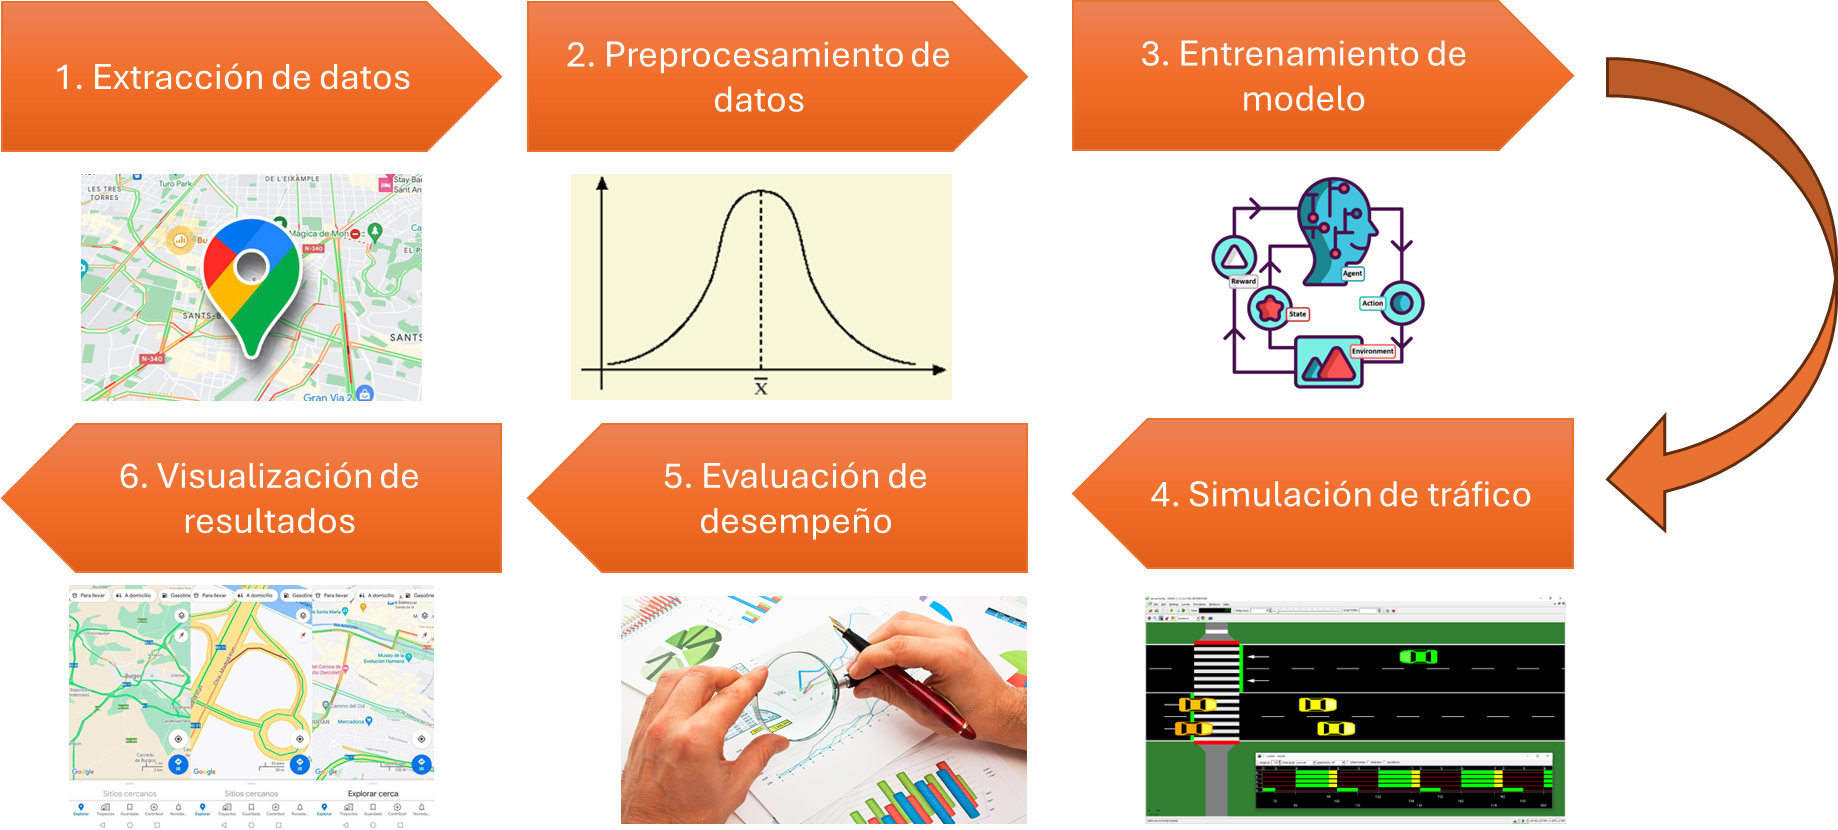
\includegraphics[width=1\linewidth]{metodologia.png}
    \caption{Metodología del proceso}
    \label{metproc}
\end{figure}

\subsection{Extracción de datos}

El primer paso de la metodología consiste en la recopilación de datos históricos y en tiempo real sobre el tráfico vehicular en las intersecciones seleccionadas de la avenida Caminos del Inca. Este proceso garantiza la obtención de información precisa y representativa para el diseño y validación del modelo de aprendizaje por refuerzo.

La recopilación de datos se llevará a cabo mediante APIs de servicios de navegación como Google Maps y Waze, que proporcionan información detallada sobre tiempos de espera, densidad vehicular y velocidades promedio en las intersecciones clave. Estos datos serán recolectados durante un período de observación de cuatro a seis semanas, abarcando tanto horas pico como no pico, para garantizar la representatividad de las diferentes condiciones de tráfico.

Además, se utilizarán herramientas de cartografía en línea como Google Maps Street View y OpenStreetMap para identificar la ubicación exacta de los semáforos en las intersecciones seleccionadas. Esta información será complementada con datos abiertos proporcionados por el municipio de Santiago de Surco, en caso de estar disponibles, para corroborar la existencia y configuración de la infraestructura semafórica.

Finalmente, se llevará a cabo un proceso de validación de los datos recolectados mediante el contraste con informes previos de tráfico y estudios de movilidad realizados en la zona. Esto asegurará que los datos utilizados sean confiables y adecuados para la simulación computacional y el entrenamiento del modelo.

\subsection{Preprocesamiento de datos}

El preprocesamiento de datos es un paso crucial para garantizar la calidad y la usabilidad de la información recolectada. Este proceso tiene como objetivo limpiar, transformar y estructurar los datos recopilados de las APIs y herramientas de navegación para que puedan ser utilizados de manera eficiente en la simulación y el entrenamiento del modelo de aprendizaje por refuerzo.

Inicialmente, los datos serán revisados para detectar inconsistencias, valores atípicos y datos faltantes. Se utilizarán técnicas de interpolación y sustitución para completar los valores ausentes y normalizar las métricas obtenidas, como los tiempos de espera, densidad vehicular y velocidades promedio. Esta normalización garantizará que los datos estén dentro de un rango uniforme, facilitando el entrenamiento del modelo.

Posteriormente, se estructurarán los datos en un formato compatible con el simulador SUMO y los algoritmos de aprendizaje por refuerzo. Esto incluye la conversión de los datos de tráfico en entradas específicas para el modelo, como estados (densidad vehicular en cada dirección), acciones (duración de las fases de semáforo) y recompensas (reducción de tiempos de espera y longitud de colas).

Finalmente, se realizará una segmentación temporal de los datos para analizar patrones de tráfico diferenciados entre horas pico y no pico. Esta segmentación permitirá entrenar el modelo bajo escenarios variados, mejorando su capacidad de generalización y adaptabilidad. Los datos procesados serán almacenados en un repositorio estructurado para su posterior uso en la etapa de simulación y modelado.

\subsection{Entrenamiento de modelo}

El entrenamiento del modelo se lleva a cabo utilizando un marco de aprendizaje por refuerzo profundo (DRL), donde cada semáforo de las intersecciones seleccionadas se representa como un agente independiente. Este agente interactúa con su entorno (condiciones de tráfico) y aprende políticas óptimas a través de un proceso iterativo de prueba y error, con el objetivo de reducir el tiempo de espera promedio y optimizar el flujo vehicular.

Para este proceso, se empleará el simulador SUMO (Simulation of Urban MObility), que permite modelar con precisión las interacciones de los vehículos y la infraestructura semafórica en escenarios urbanos. El entorno de simulación replica las condiciones de tráfico observadas en la avenida Caminos del Inca, integrando los datos procesados previamente. Este simulador proporciona un marco controlado y escalable para probar diversas configuraciones de tráfico.

El modelo se entrenará con un algoritmo de aprendizaje por refuerzo, como el Deep Q-Network (DQN), que utiliza una red neuronal profunda para aproximar las recompensas esperadas de cada acción posible. Estas acciones incluyen cambios en la duración de las fases de luz verde, amarilla y roja en cada semáforo. El entrenamiento se ejecutará en iteraciones múltiples, cada una representando un episodio en el simulador, donde el agente observa el estado del tráfico, toma decisiones y ajusta sus políticas basándose en la retroalimentación obtenida.

Durante el proceso de entrenamiento, se empleará un enfoque multiagente, permitiendo que los semáforos colaboren y compartan información para optimizar el rendimiento global del sistema de tráfico. Además, se monitorearán métricas clave como la velocidad promedio de convergencia, el tiempo de espera y la longitud de las colas vehiculares, ajustando los hiperparámetros del modelo (como la tasa de aprendizaje y el factor de descuento) para maximizar su eficiencia.

El resultado de esta etapa será un modelo entrenado capaz de operar en condiciones reales o simuladas, adaptándose dinámicamente a las variaciones del tráfico y mejorando los indicadores clave de desempeño definidos en el estudio.

\subsection{Simulación de tráfico}

La etapa de simulación de tráfico es fundamental para validar el modelo entrenado y analizar su desempeño en escenarios controlados que replican las condiciones reales de la avenida Caminos del Inca. Esta etapa se lleva a cabo utilizando el simulador SUMO (Simulation of Urban MObility), el cual permite modelar redes de tráfico urbanas con alto grado de precisión y flexibilidad.

La simulación se inicia configurando el entorno con los datos procesados previamente, incluyendo las características específicas de las intersecciones seleccionadas, como el número de carriles, las direcciones del flujo vehicular y los patrones observados en horarios pico y no pico. Asimismo, se introducen escenarios variables, como fluctuaciones en la densidad vehicular y eventos aleatorios que puedan alterar el tráfico, para evaluar la capacidad de adaptación del modelo.

El proceso de simulación se repite en múltiples episodios para obtener resultados estadísticamente significativos. Cada iteración permite ajustar los parámetros del modelo y evaluar su estabilidad y rendimiento bajo condiciones diversas. Al finalizar la simulación, se compararán los resultados obtenidos con el sistema tradicional de control fijo de semáforos, estableciendo diferencias en términos de eficiencia y reducción de congestión vehicular.

El uso de herramientas de visualización integradas en SUMO facilita la representación gráfica de los patrones de tráfico antes y después de la implementación del modelo. Estas visualizaciones son esenciales para interpretar los resultados y comunicar de manera efectiva el impacto del sistema propuesto.

\subsection{Evaluación de desempeño}

La etapa de evaluación del modelo tiene como objetivo medir el impacto del sistema de gestión inteligente de semáforos en la mejora del tráfico vehicular en las intersecciones seleccionadas. Este análisis se realiza utilizando métricas clave, las cuales permiten cuantificar la efectividad del modelo propuesto frente al sistema tradicional de control fijo.

Las métricas utilizadas son:
\begin{itemize}
    \item Tiempo promedio de espera por vehículo: Evalúa la reducción del tiempo que los vehículos permanecen detenidos en las intersecciones. Una disminución significativa en esta métrica indica una mejora en la eficiencia del flujo vehicular.
    \item Longitud promedio de las colas: Mide el nivel de congestión en las intersecciones. Esta métrica es crucial para identificar la capacidad del modelo para descongestionar puntos críticos del tráfico.
    \item Volumen vehicular procesado: Determina la cantidad de vehículos que el sistema puede gestionar en un período específico. Este indicador es esencial para evaluar la capacidad de las intersecciones bajo diferentes niveles de demanda vehicular.
\end{itemize}

La evaluación se llevará a cabo en tres etapas principales:

\begin{itemize}
    \item Comparación directa con el sistema tradicional: Se realizarán simulaciones bajo las mismas condiciones de tráfico utilizando tanto el modelo inteligente como el sistema de control fijo. Las diferencias en las métricas clave permiten cuantificar la mejora lograda.
    \item Análisis de escenarios extremos: Se evaluará el desempeño del modelo en condiciones de alta demanda vehicular (horas pico) y bajo tráfico (horas no pico). Esto asegurará que el modelo sea robusto y adaptable a diferentes contextos.
    \item Estadísticas de rendimiento agregado: Los resultados de múltiples simulaciones se promediarán para obtener valores representativos de cada métrica. Se emplean herramientas estadísticas para validar la significancia de las mejoras observadas.
\end{itemize}

\subsection{Visualización de resultados}

La visualización de resultados es una etapa clave en la metodología, ya que permite interpretar de manera clara y comprensible el impacto del modelo de gestión inteligente de semáforos sobre el tráfico vehicular. Para ello, se generarán gráficos comparativos y representaciones visuales que muestren el comportamiento del tráfico antes y después de la implementación del modelo propuesto.

Se elaborarán gráficos de barras y líneas que representen las métricas clave, como el tiempo promedio de espera, longitud de las colas y volumen vehicular procesado. Estos gráficos permitirán observar visualmente las mejoras en el flujo de tráfico bajo el nuevo sistema frente al sistema tradicional de semáforos. Por ejemplo, un gráfico de barras podría mostrar la comparación de los tiempos de espera en las intersecciones durante las horas pico antes y después de la implementación del modelo de aprendizaje por refuerzo, destacando la reducción en los tiempos de espera promedio.

Se utilizarán diagramas de dispersión y mapas de calor para visualizar la distribución del tráfico a lo largo de la avenida en diferentes horarios del día. Estos mapas facilitarán la identificación de puntos críticos y mostrarán cómo la distribución del tráfico cambia con el ajuste dinámico de los semáforos. Además, los mapas de flujo vehicular podrán ilustrar el impacto en la fluidez del tráfico en intersecciones claves, destacando las áreas con mejoras significativas en la capacidad de procesamiento de vehículos.

A través de gráficos de líneas y áreas, se podrán representar las variaciones en la longitud de las colas en tiempo real, lo que permitirá observar cómo el modelo responde a fluctuaciones en la densidad vehicular. Este tipo de visualización es crucial para entender la efectividad del sistema en escenarios de congestión extrema y su capacidad para reducir los cuellos de botella en las intersecciones.

Se desarrollarán gráficos de series temporales que muestren la evolución de los tiempos de espera y la fluidez vehicular durante las horas pico y no pico. Esto ayudará a resaltar las diferencias en el rendimiento del sistema durante diferentes períodos del día y evaluar la adaptabilidad del modelo a las variaciones en la demanda del tráfico.

Estos gráficos y representaciones serán herramientas clave no solo para la interpretación interna de los resultados, sino también para la presentación de los hallazgos a los tomadores de decisiones y otros interesados, facilitando la justificación de la efectividad del sistema propuesto.

\section{Cronograma y presupuesto}

En esta sección se observa el cronograma cumplido para el desarrollo de la primera parte de la presente tesis.

\begin{figure}[H]
    \centering
    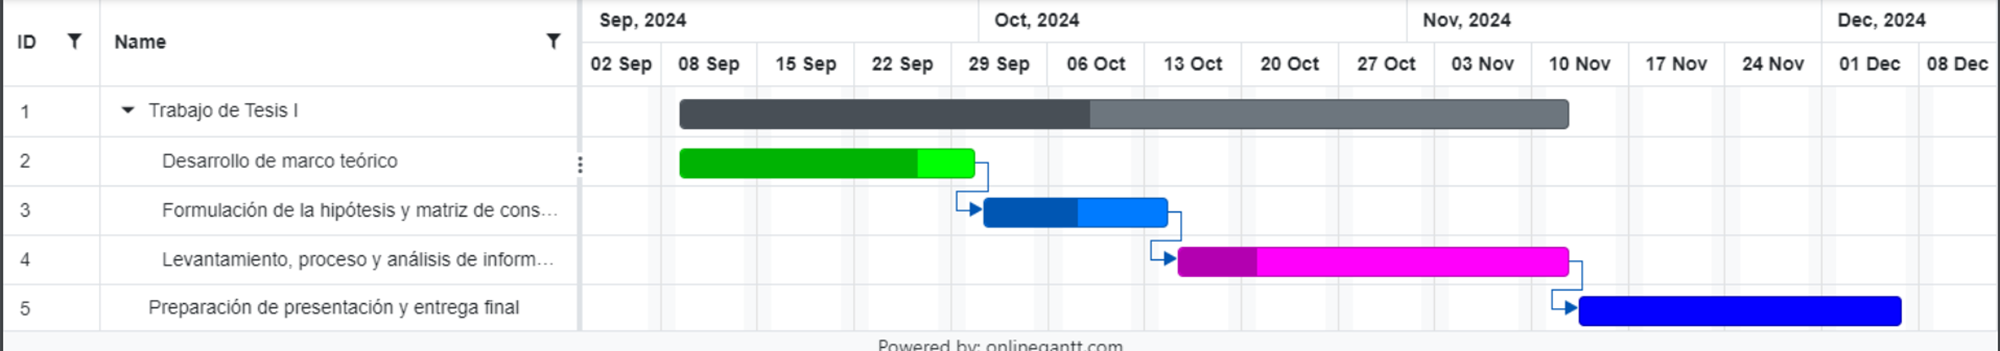
\includegraphics[width=1\linewidth]{gantt.png}
    \caption{Cronograma de primera parte}
    \label{fig:enter-label}
\end{figure}

Por otro lado, se presenta el presupuesto con los principales gastos asociados al desarrollo del modelo.

\begin{table}[H]
	\caption[Presupuesto]{Presupuesto de la investigación.}
	\label{3:table1}
	\centering
	\small
	\begin{tabular}{llll}
		\specialrule{.1em}{.05em}{.05em}
		{Grupo} & {Item} & {Costo (soles)} & {Subtotal} \\
		\specialrule{.1em}{.05em}{.05em}
	{Recursos} & {Equipo de cómputo} & {S/ 3,000.00} & {S/ 3,000.00} \\
		\cline{1-4}
        {Software} & {Simulador} & {S/ 100.00} & {} \\
		{} & {Mantenimiento de equipo} & {S/ 300.00} & {S/ 400.00} \\ % & {S/ 5,274.15} \\
		\cline{1-4}
		\multirow{2}{4cm}

	\end{tabular}
	\begin{flushleft}	
		\small Fuente: Elaboración propia.
	\end{flushleft}
\end{table}




%\input{4/desarrollo}
%\input{5/resultados} %Esta es la conclusión
%\input{6/conclusion}
% %%Bibliografia
%\bibliographystyle{apalike} % No funciona
%\renewcommand{\bibname}{BIBLIOGRAFÍA} % changes the header; default: Bibliography

\printbibliography[heading=bibintoc,title={Referencias}]
%\bibliography{biblio/references} % adjust this to fit your BibTex file

%%Anexos
%\appendix
%\renewcommand{\appendixname}{Anexo} %Esto es para las paginas
%\renewcommand{\appendixtocname}{Anexos} %Esto es para el indice
%\renewcommand{\appendixpagename}{Anexos}
%\clearpage
%\addappheadtotoc
%\appendixpage
%%\begin{appendices}

\appendix
%\chapter*{ANEXOS}% If \appendix doesn't insert a \chapter
%\addcontentsline{toc}{chapter}{ANEXOS}% Print Appendix in ToC
\setcounter{section}{0}% Reset numbering for sections
\renewcommand{\thesection}{\Alph{section}}% Adjust section printing (from here onward)
	
	\section{Árbol de Problemas}
	%\chapter*{Árbol de Problemas}
	%\addcontentsline{toc}{section}{Árbol de Problemas}
	%\renewcommand{\thechapter}{A}
	\label{anexo1}
	\begin{figure}[h]
		\begin{center}
			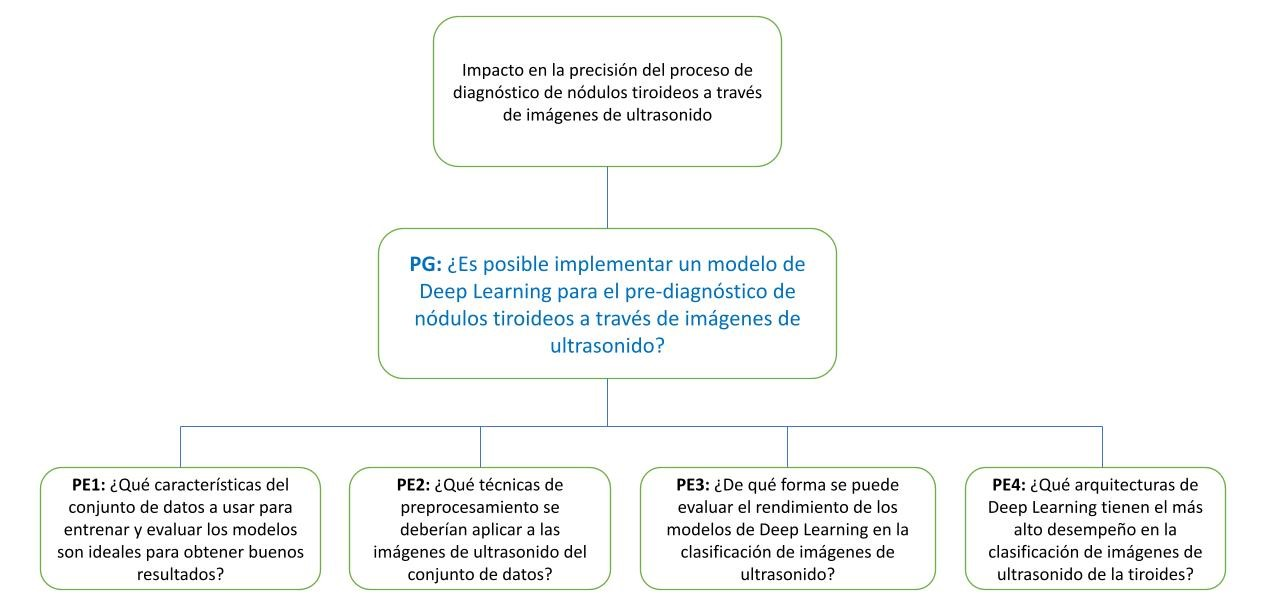
\includegraphics[width=1.00\textwidth]{anexos/arb_problemas.jpg}
			%\caption{Fuente: Elaboración propia}
		\end{center}
	\end{figure}
	\clearpage
	
	\section{Árbol de Objetivos}
	%\chapter*{Árbol de Objetivos}
	%\addcontentsline{toc}{section}{Árbol de Objetivos}
	%\renewcommand{\thechapter}{A}
	\label{anexo2}
	\begin{figure}[h]
		\begin{center}
			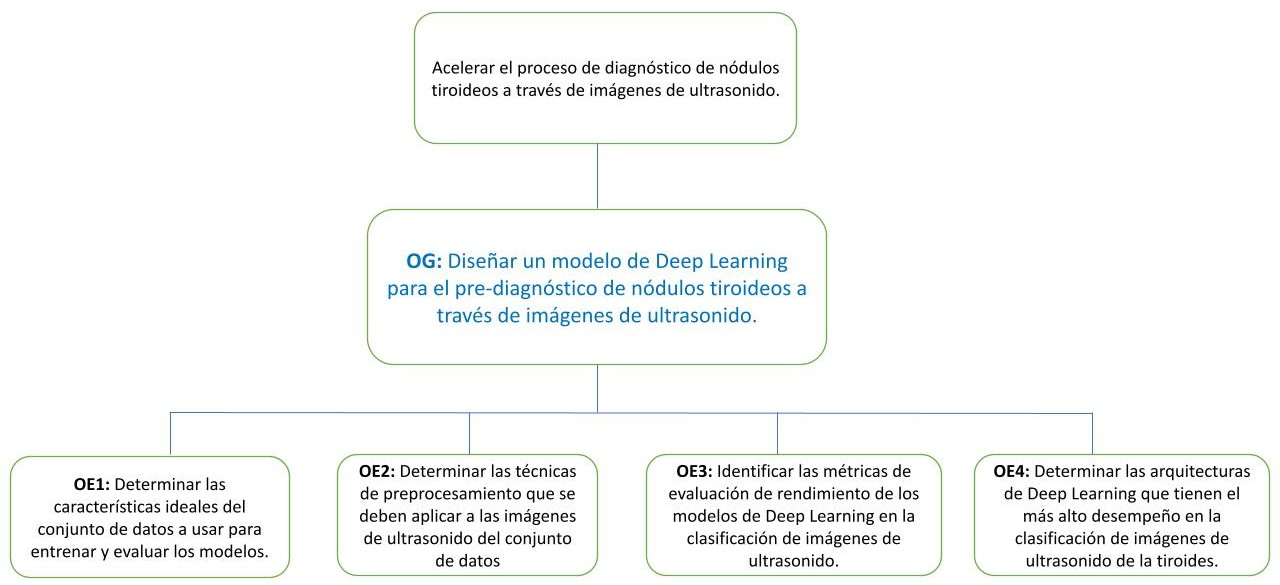
\includegraphics[width=1.00\textwidth]{anexos/arb_objetivos.jpg}
			%\caption{Fuente: Elaboración propia}
		\end{center}
	\end{figure}
	\clearpage
	
	\begin{landscape}
		\section{Matriz de Consistencia}
		\label{anexo3}
		\begin{longtable}{ p{3.5cm}p{3.5cm}p{3.5cm}p{3cm}p{3cm}p{3cm}p{3cm} }
			%\centering
			\small
			\tabularnewline \specialrule{.1em}{.05em}{.05em}
			\centering{Título de la tesis} & \multicolumn{6}{p{15cm}}{Diseño de un modelo de Deep Learning para el pre-diagnóstico de nódulos tiroideos a través de imágenes de ultrasonido}
			\tabularnewline \specialrule{.1em}{.05em}{.05em}
			\Centering{Problema General}& \Centering{Objetivo General} & \Centering{Hipótesis General} & \Centering{Variables} & \Centering{Método} \\
			\specialrule{.1em}{.05em}{.05em}
			{\ProblemaGeneral} & { \ObjetivoGeneral} & {\HipotesisGeneral} & {

				Dependiente: Pre-diagnóstico de nódulos tiroideos. Independiente: Modelo de Deep Learning.

			} \\
			\cline{1-4}
			\Centering {Problemas Específicos} & \Centering {Objetivos Específicos} & \Centering {Hipótesis Específicas} & \Centering {Variables} \\ %& \Centering {Método} \\
			\cline{1-4}
			{\Pbone} & {\Objone} & {\Hone} & {

				Dependiente: Desarrollo del modelo de Deep Learning. Independiente: Las características del conjunto de datos.

			} & \multirow{6}{3cm}{
				
				\centering Tipo de Investigación: Experimental. Alcance de la investigación: Explicativo.
			
			} \\
			\cline{1-4}
			{\Pbtwo} & {\Objtwo} & {\Htwo}  & {
				
				Dependiente: Desempeño del modelo de Deep Learning. Independiente: Técnicas de preprocesamiento.
			
			} \\ % & {aa } \\
			\cline{1-4}
			{\Pbthree} & {\Objthree} & {\Hthree}  & { 
				
				Dependiente: Comparación de modelos en la tarea de clasificación de imágenes de ultrasonido. Independiente: Las métricas de evaluación de rendimiento.
				
			} \\ % & {aa } \\
			\cline{1-4}
			{\Pbfour} & {\Objfour} & {\Hfour}  & { 
				
				Dependiente: Desempeño en la clasificación de imágenes de ultrasonido. Independiente: Las arquitecturas de Deep Learning.
			
			} \\ % & { aa} \\
			\specialrule{.1em}{.05em}{.05em}
		\end{longtable}
	\end{landscape}
	\clearpage
	
\end{document}